\section{Results} \label{results}
In this section we show the results for our methodology. First we illustrate the good performance of our classifiers, both \ac{RF} and \ac{KNN}. Then we can use them to construct Bayesian probabilities according to their output and finally evaluate new events, synthetic and real.

\subsection{Performance of the algorithms}
We measure the performance of our algorithms by the true positive and false positive rates, drawn as \textit{Receiver Operating Characteristic} (ROC) curves. They show the variation of the true-positive rate  with the false-positive rate given a certain threshold for the probability. The better the classifier, the steeper the curve,  achieving a greater number of true positives with few false classifications. We use the testing set that with synthetic data from LVK's O2 run. 

\begin{figure*}%[h]
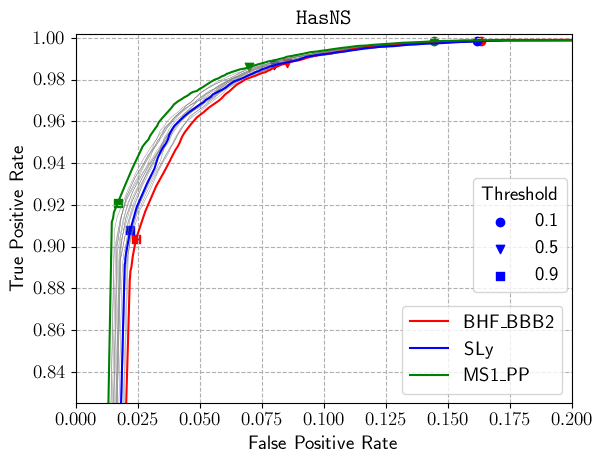
\includegraphics[width=0.45\linewidth]{roc_testing_KNN_NS}
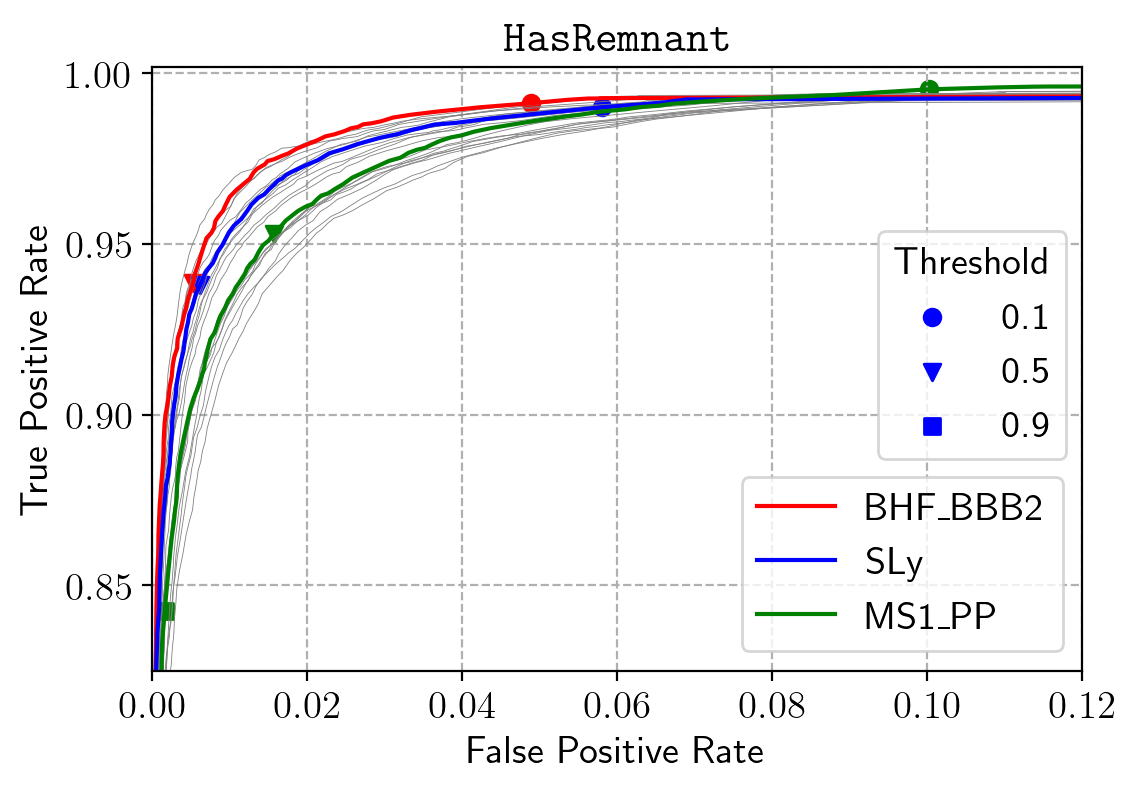
\includegraphics[width=0.45\linewidth]{roc_testing_KNN_REM}
\caption{ROC curves for the testing dataset for \ac{KNN}
    classifier. All 23 EoS shown in grey, in color the EoSs with minimum and
    maximum mass, along commonly used SLy.}
\label{fig:rocO2_KNN}
\end{figure*}

\begin{figure*}%[h]
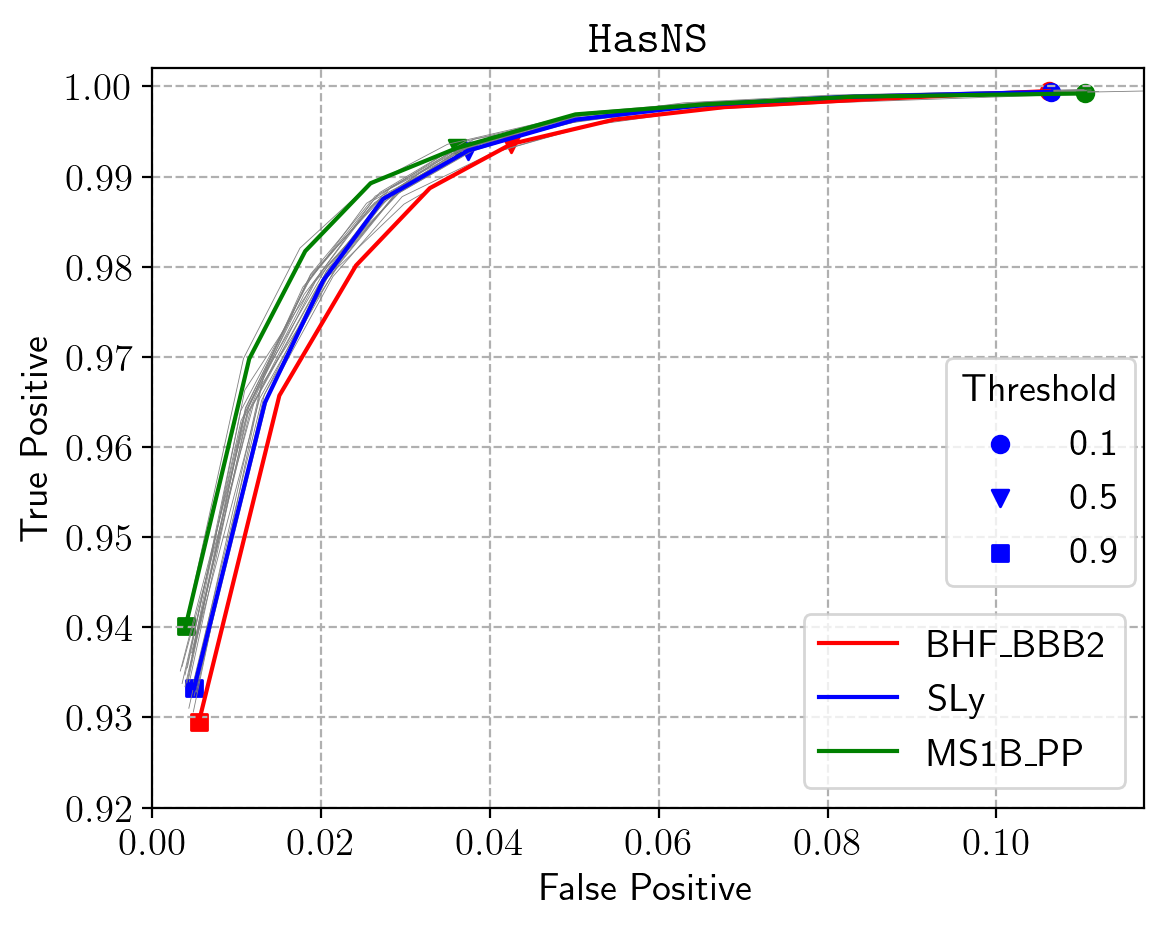
\includegraphics[width=0.45\linewidth]{ROC_O2testing_NS_RF}
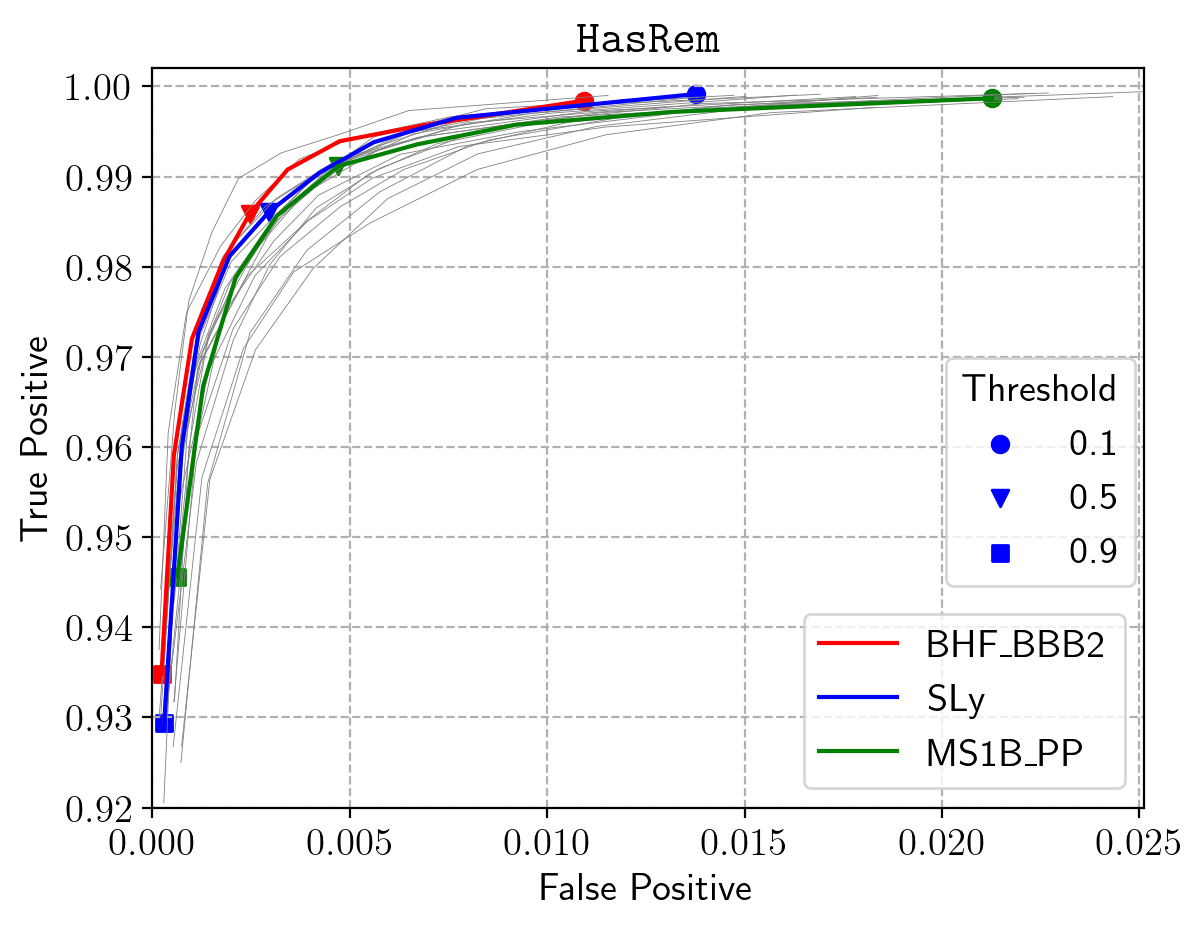
\includegraphics[width=0.45\linewidth]{ROC_O2testing_REM_RF}
\caption{ROC curves for the testing dataset for \ac{RF} classifier. All 23 EoS shown in grey, in color the EoSs with minimum and maximum mass, along commonly used SLy. \mmt{[MMT: Please unify x axis and size of the plot.]}}
\label{fig:rocO2_RF}
\end{figure*}

The curves for \ac{KNN} and \ac{RF} are in Figures~\ref{fig:rocO2_KNN}
and~\ref{fig:rocO2_RF}, respectively. We show the curves for each EOS, but we
highlight 3 concrete cases: BHF BBB2 (EOS with lowest maximum mass for the NS),
MS1 PP (EOS with largest maximum mass for the NS) and SLy (the most accepted
case \mmt{[?]}). The results are consistent among all equations of state and
depict a true positive rate around $0.99$ for a threshold of $0.5$ and for both labels, but with a higher false positive rate in the case of \hasns, which means that the algorithms perform better when dealing with \hasrem.

Both algorithms perform similarly on the testing dataset, but \ac{RF} gives slightly higher true positive rates and lower false positive rates for a given threshold. 

\todo{UNIFY AXIS AND SIZE OF FIGURES}

\subsection{Computation of the probabilities}

Once the algorithms are trained and tested, we compute the Bayesian
probabilities defined in the Section~\ref{bayesian_probs}, in terms of the 
output of the algorithms (fractions of neighbors and fractions of trees, 
respectively). In order to obtain the probabilities given in 
Equations~\ref{bayes-hasns} and~\ref{bayes-hasrem} one needs to apply
 the algorithm on known events \mmt{[MMT: applied on O2, right?]}. 

\begin{figure*}%[h]
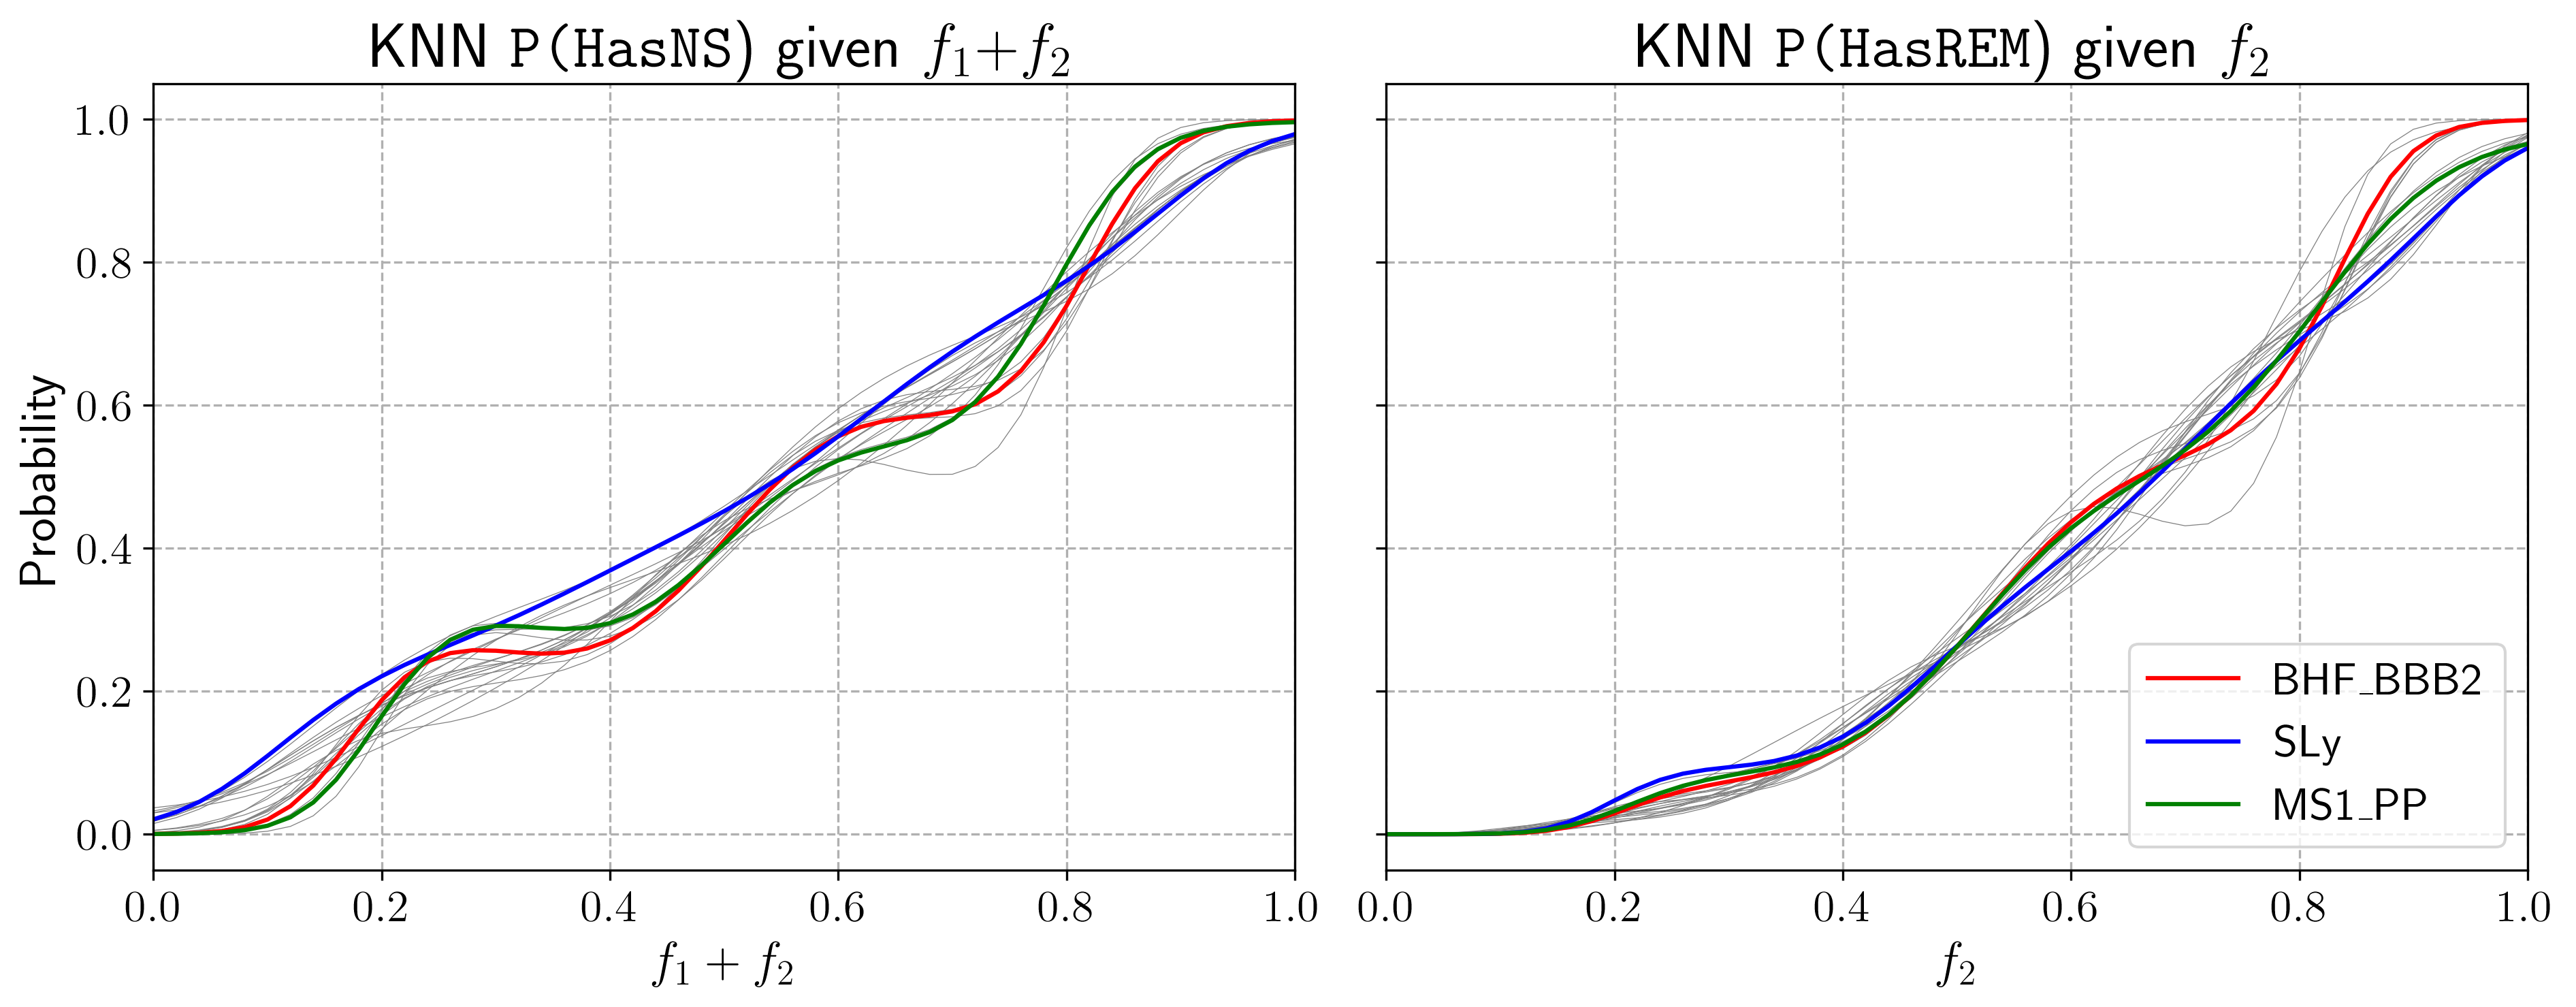
\includegraphics[width=0.65\linewidth]{KNN_3_eos_prob_plots}
\caption{.}
\label{fig:bayesian_prob_fits_KNN}
\end{figure*}

\begin{figure*}%[h]
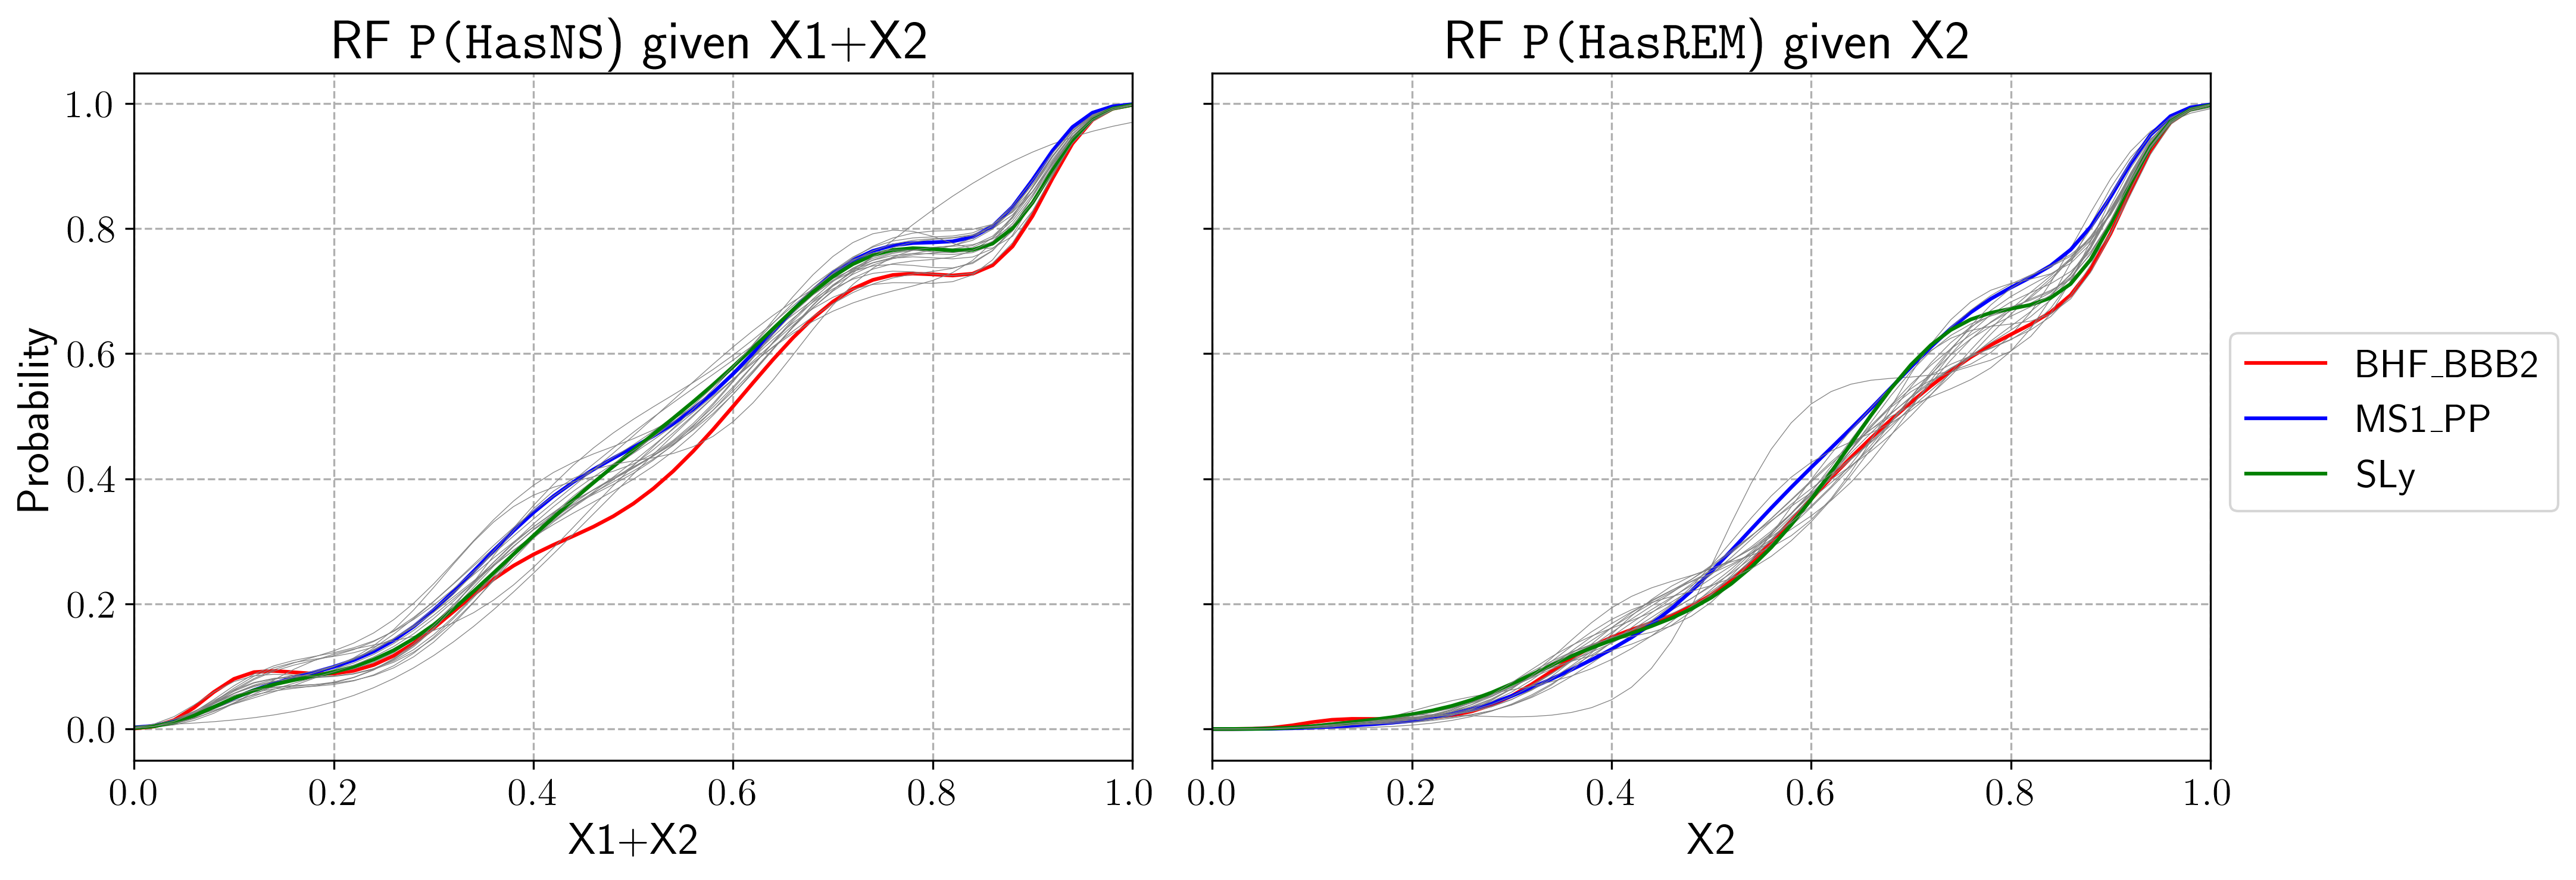
\includegraphics[width=0.65\linewidth]{RF_3_eos_prob_plots}
\caption{}
\label{fig:bayesian_prob_fits_RF}
\end{figure*}

In Figs.~\ref{fig:bayesian_prob_fits_KNN} and~\ref{fig:bayesian_prob_fits_RF}, 
we show the fits of  the results with a Gaussian Process Regression,
performed as explained in the Section~\ref{bayesian_probs}. In this figures we show
the fits for each EOS, but one can always get a single marginalized probability
applying the Bayes factors. The fitted curves are monotonic and have a
sigmoid-like shape, but that depends on the choice of the EOS. Both \ac{KNN}
and \ac{RF} give fits that have a similar shape. Indeed, both show a slower
increase of $P(\hasrem)$ for a low fraction $f_2$ compared to $P(\hasns)$.
However, \ac{RF} shows a small plateau on the $P(\hasns)$ (and also on
$P(\hasrem)$) for fractions of trees around $0.8$, and that is something that
\ac{KNN} does not reproduce. We highlight the same equations of state as in
Figs.~\ref{fig:rocO2_KNN} and~\ref{fig:rocO2_RF}.

\subsection{Performance on new events}

As stated in the Section~\ref{bayesian_probs}, the fits of the probabilities
$P_J(I|{\bf A}_{\bf X})$ for each EOS ($J=1,\dots 23$) can be tabulated and
used to compute the marginalized probabilities $P_M(\hasns|{\bf A}_{\bf E})$
and $P_M(\hasrem|{\bf A}_{\bf E})$ for any new event $\bf E$ with algorithm
outcome $\bf A_{E}$.  We classify the events from MDC11 \todo{explain? or was
it explained before?} and compute the ROC curves according the ground truth of
the injected events, which can be seen in Figs.~\ref{fig:rocMDC_KNN}
and~\ref{fig:rocMDC_RF}. We separate the ROC curves for the different pipelines
involved in the dataset (GstLAL,  PyCBC~\cite{Usman:2015kfa},
SPIIR~\cite{Chu:2020pjv} and MBTA~\cite{Adams:2015ulm}). Notice that the curves are very similar even though the algorithms were trained (and also the Bayesian probabilities were fitted) using exclusively GstLAL.

Figure~\ref{fig:rocMDC_KNN} depicts the curves for \ac{KNN}.  In the case of
\hasns\ (left panel), it gives a true positive rate of $\sim 0.975$ for a
threshold of $0.5$ and less than a false positive rate of $0.2$ for all the
pipelines except of SPIIR. Regarding \hasrem\ (right panel), \ac{KNN}. gives a
false positive rate slightly higher than $0.2$ for all the pipelines except of
GstLAL when fixing the threshold to $0.5$, but the true positive rate stays
around $0.975$. In this case, SPIIR behaves similarly to the rest of the pipelines.  

In Fig.~\ref{fig:rocMDC_RF} we showcase the results for \ac{RF}.  The curves
are similar to the ones in Fig.~\ref{fig:rocMDC_KNN}, having a steeper shape for \hasns\ (left panel) and thus giving high true positive rates and low false positive rates at a given threshold. SPIIR also performs poorly for \ac{RF}. When it comes to \hasrem\ (right panel), the false positive rates increase as for \ac{KNN}, but again all the pipelines behave similarly. One can note that \ac{RF} gives slightly steeper ROC curves than \ac{KNN},  which results in higher true positive rates at lower false positive rates. 

%\begin{comment}
%performs very well for \hasns achieving a true positive rate very close to
%unity with a very small false positive rate. We observe that SPIIR pipeline
%deviates from the good behaviour. For \hasrem the overall performance is
%slightly worse, getting higher false positive rate, but in turn all
%pipelines behave equally good. In Fig.~\ref{fig:rocMDC_RF} we showcase the results for \ac{RF}. As with \ac{KNN} the results are very good, with steep ROC curves. For \hasns spiir pipeline deviates less from the rest, getting higher positive rates for the same false positives than with \ac{KNN}. In the case of \hasrem the curves of the different pipelines behave a bit more differently from each other.
%\end{comment}

\begin{figure*}%[h]
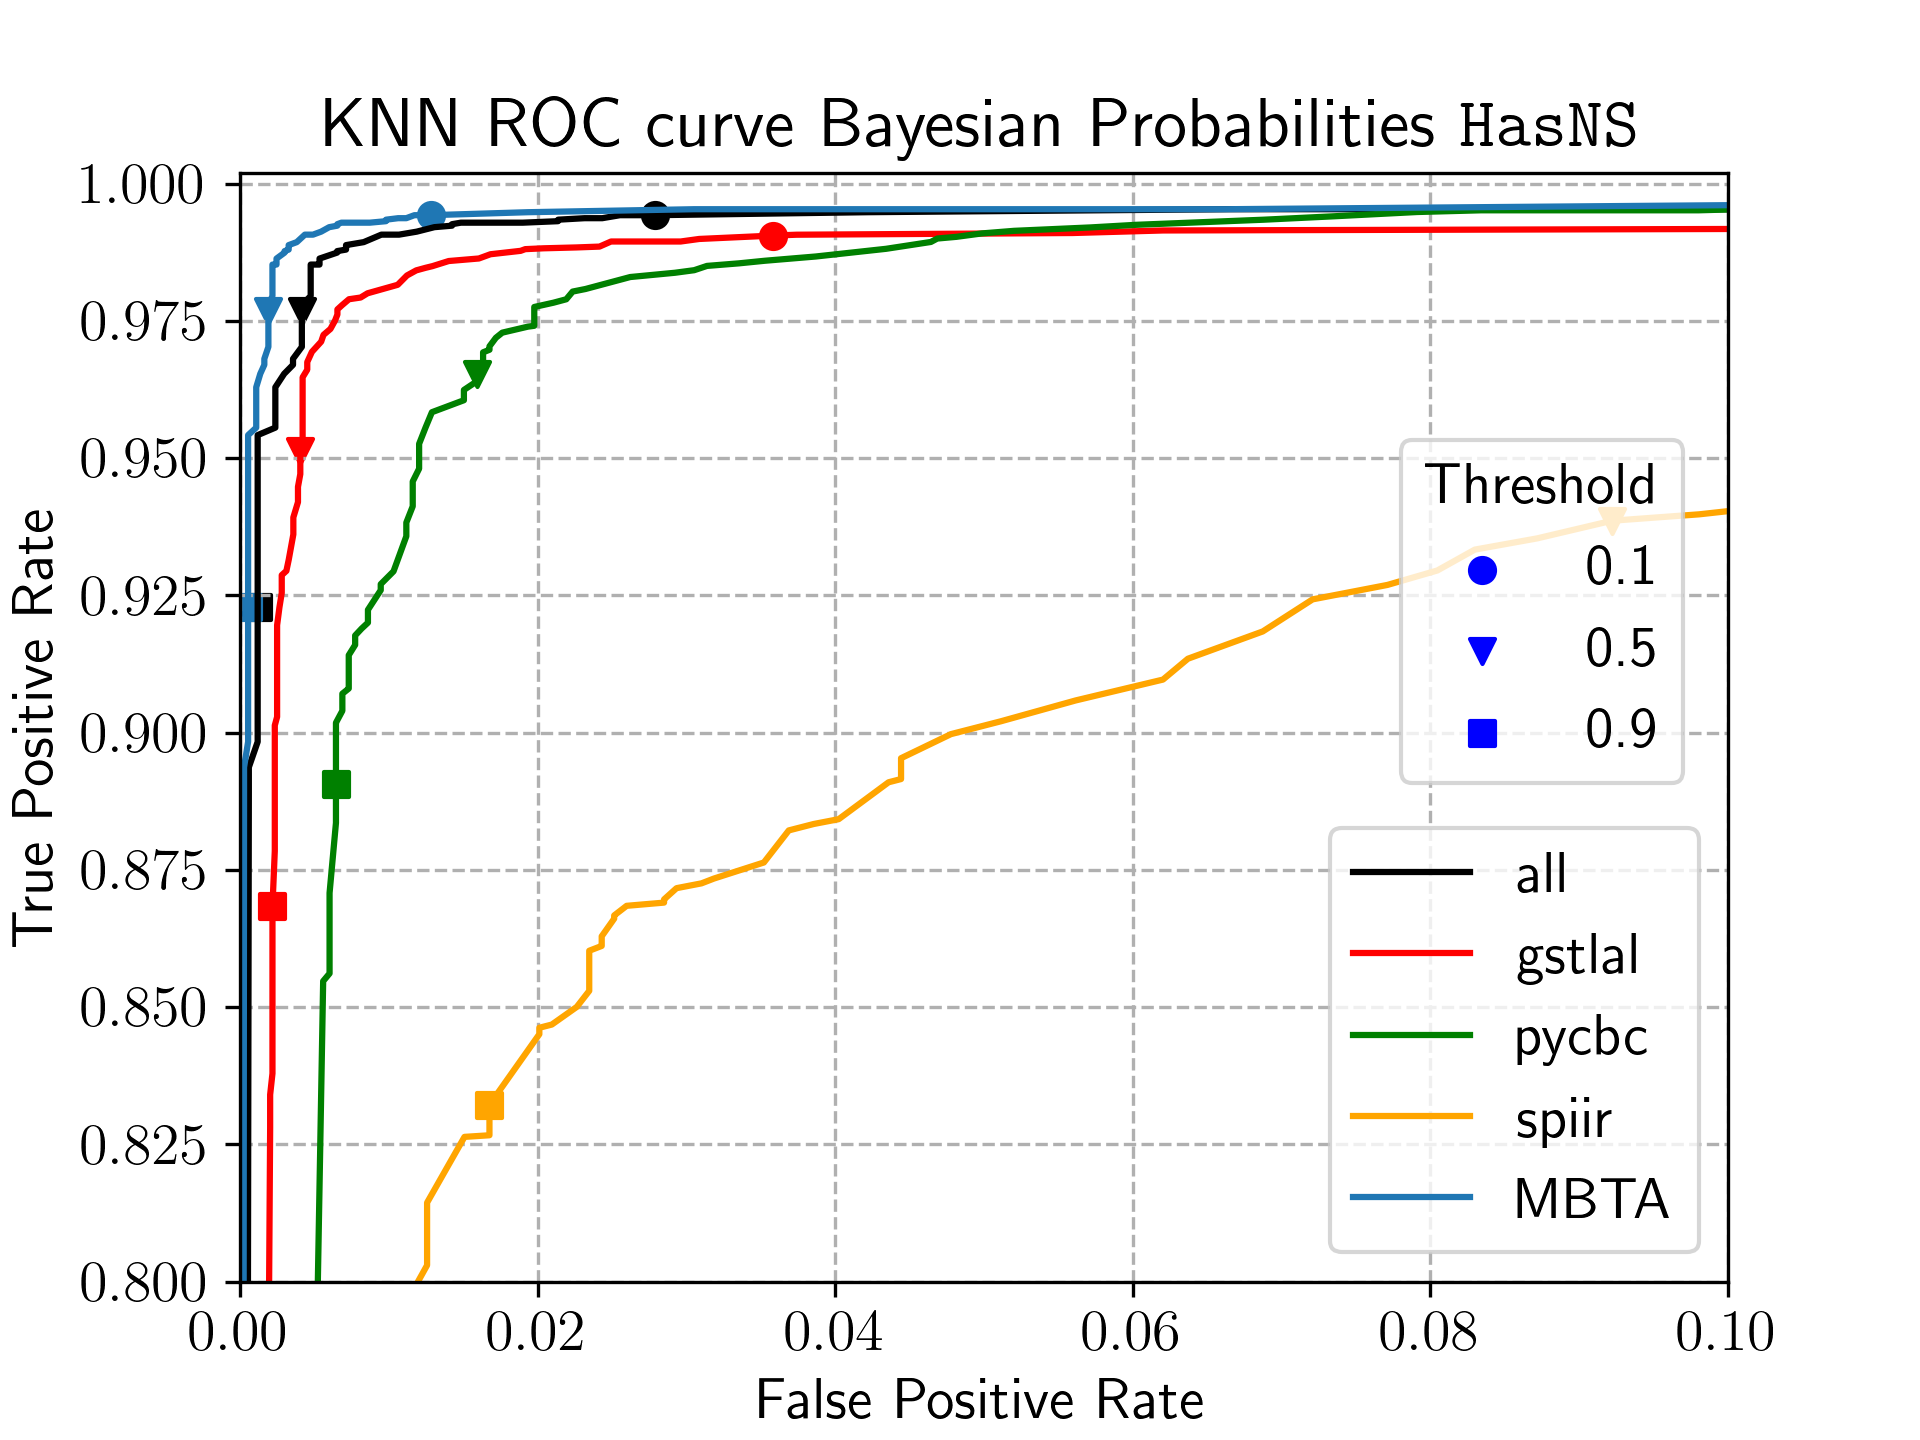
\includegraphics[width=0.45\linewidth]{KNN_bayesian_NS}
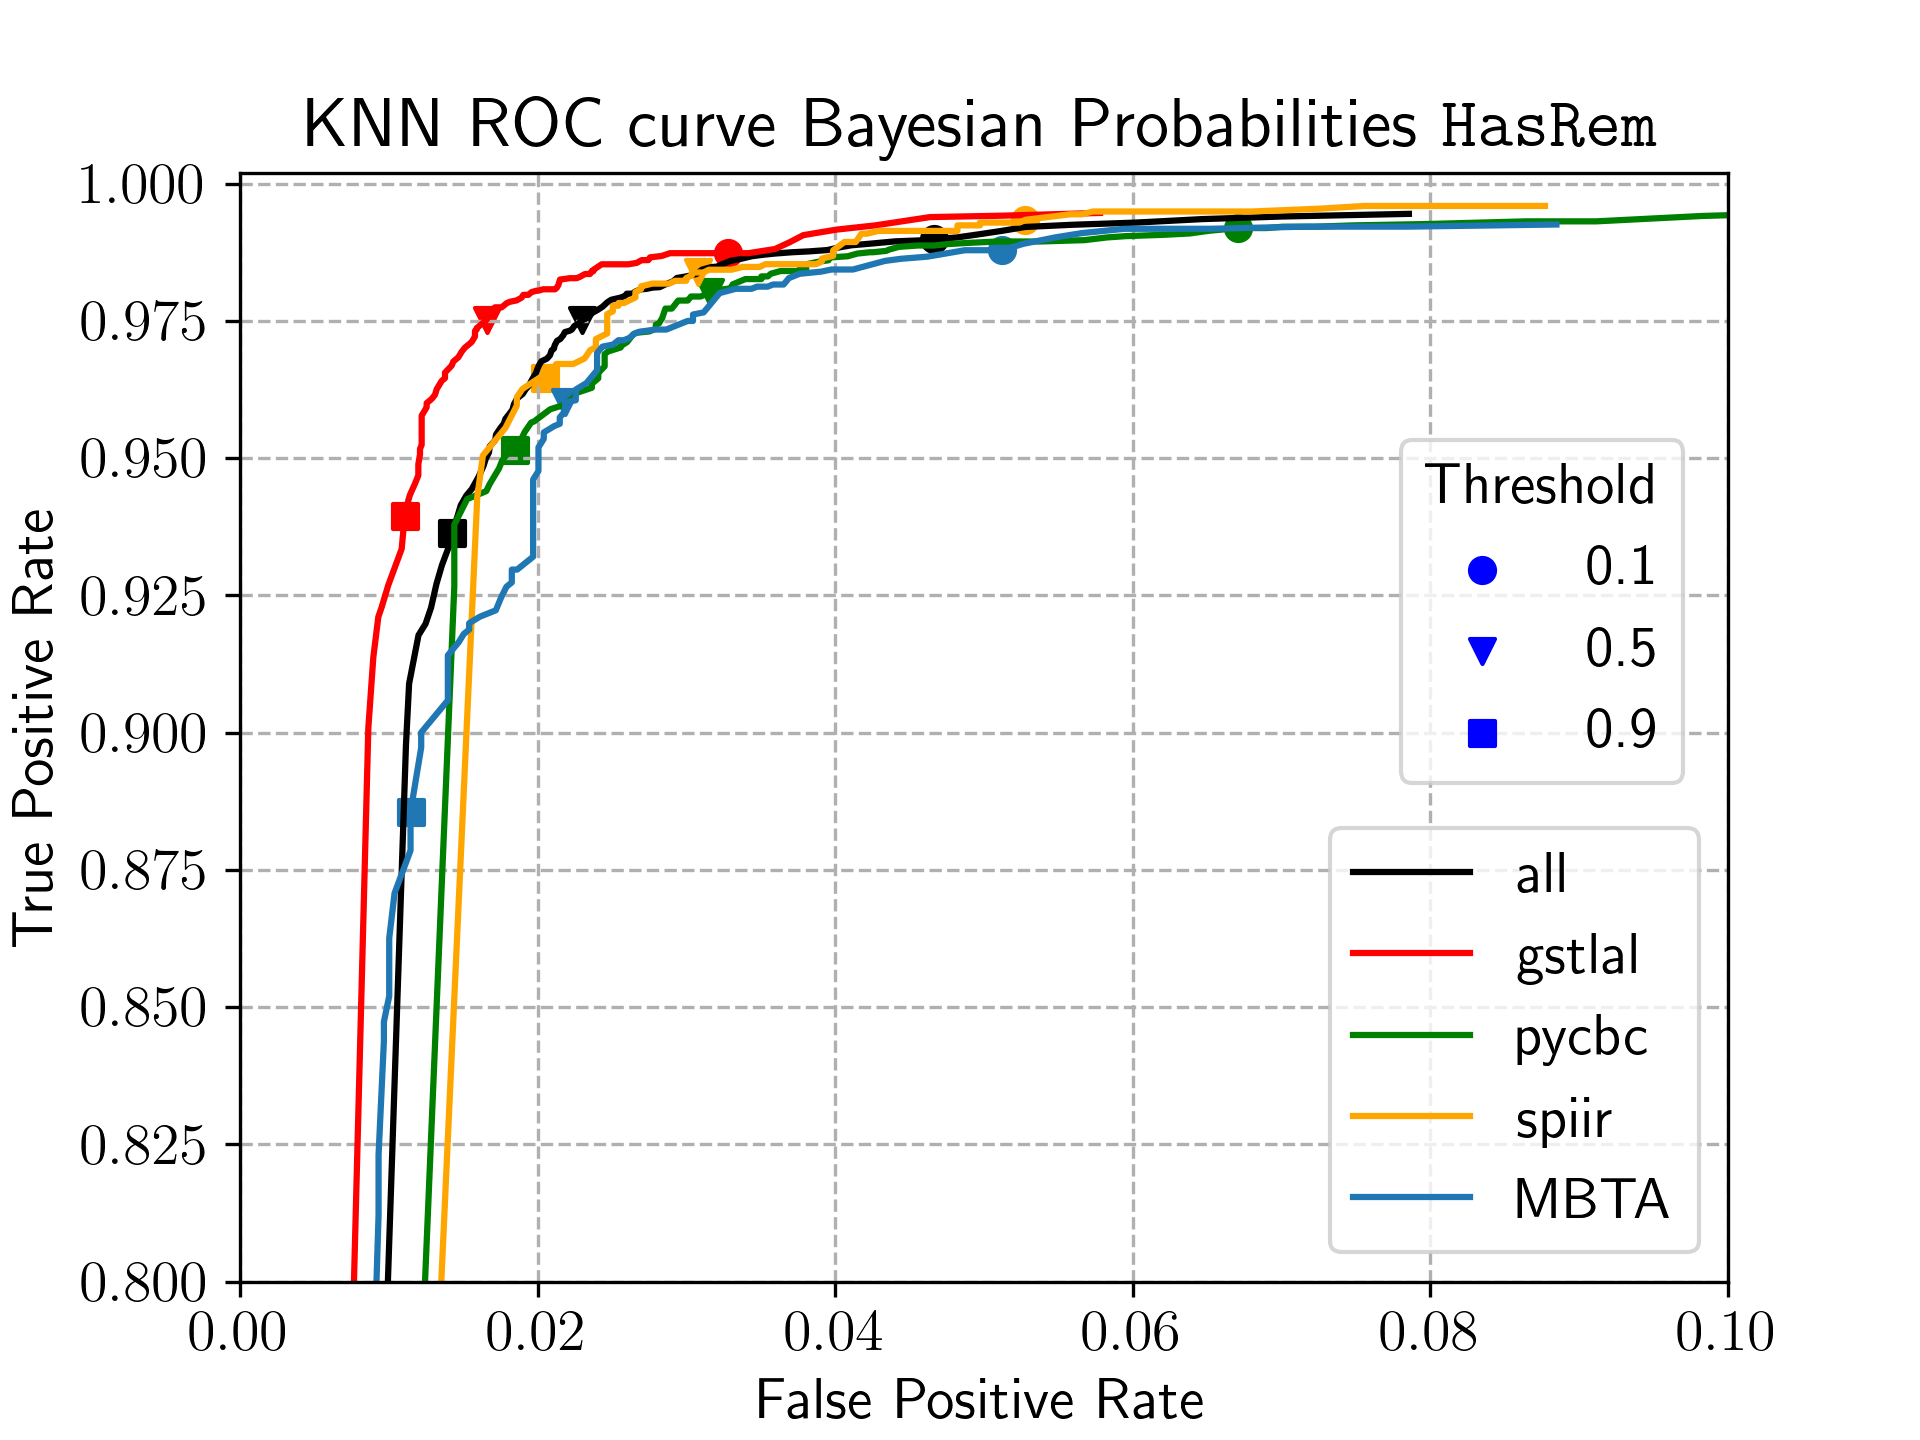
\includegraphics[width=0.45\linewidth]{KNN_bayesian_REM}
\caption{ROC curves of Bayesian probability marginalized
    for the 23 EoSs for MDC11 dataset using \ac{KNN} classifier.}
\label{fig:rocMDC_KNN}
\end{figure*}

\begin{figure*}%[h]
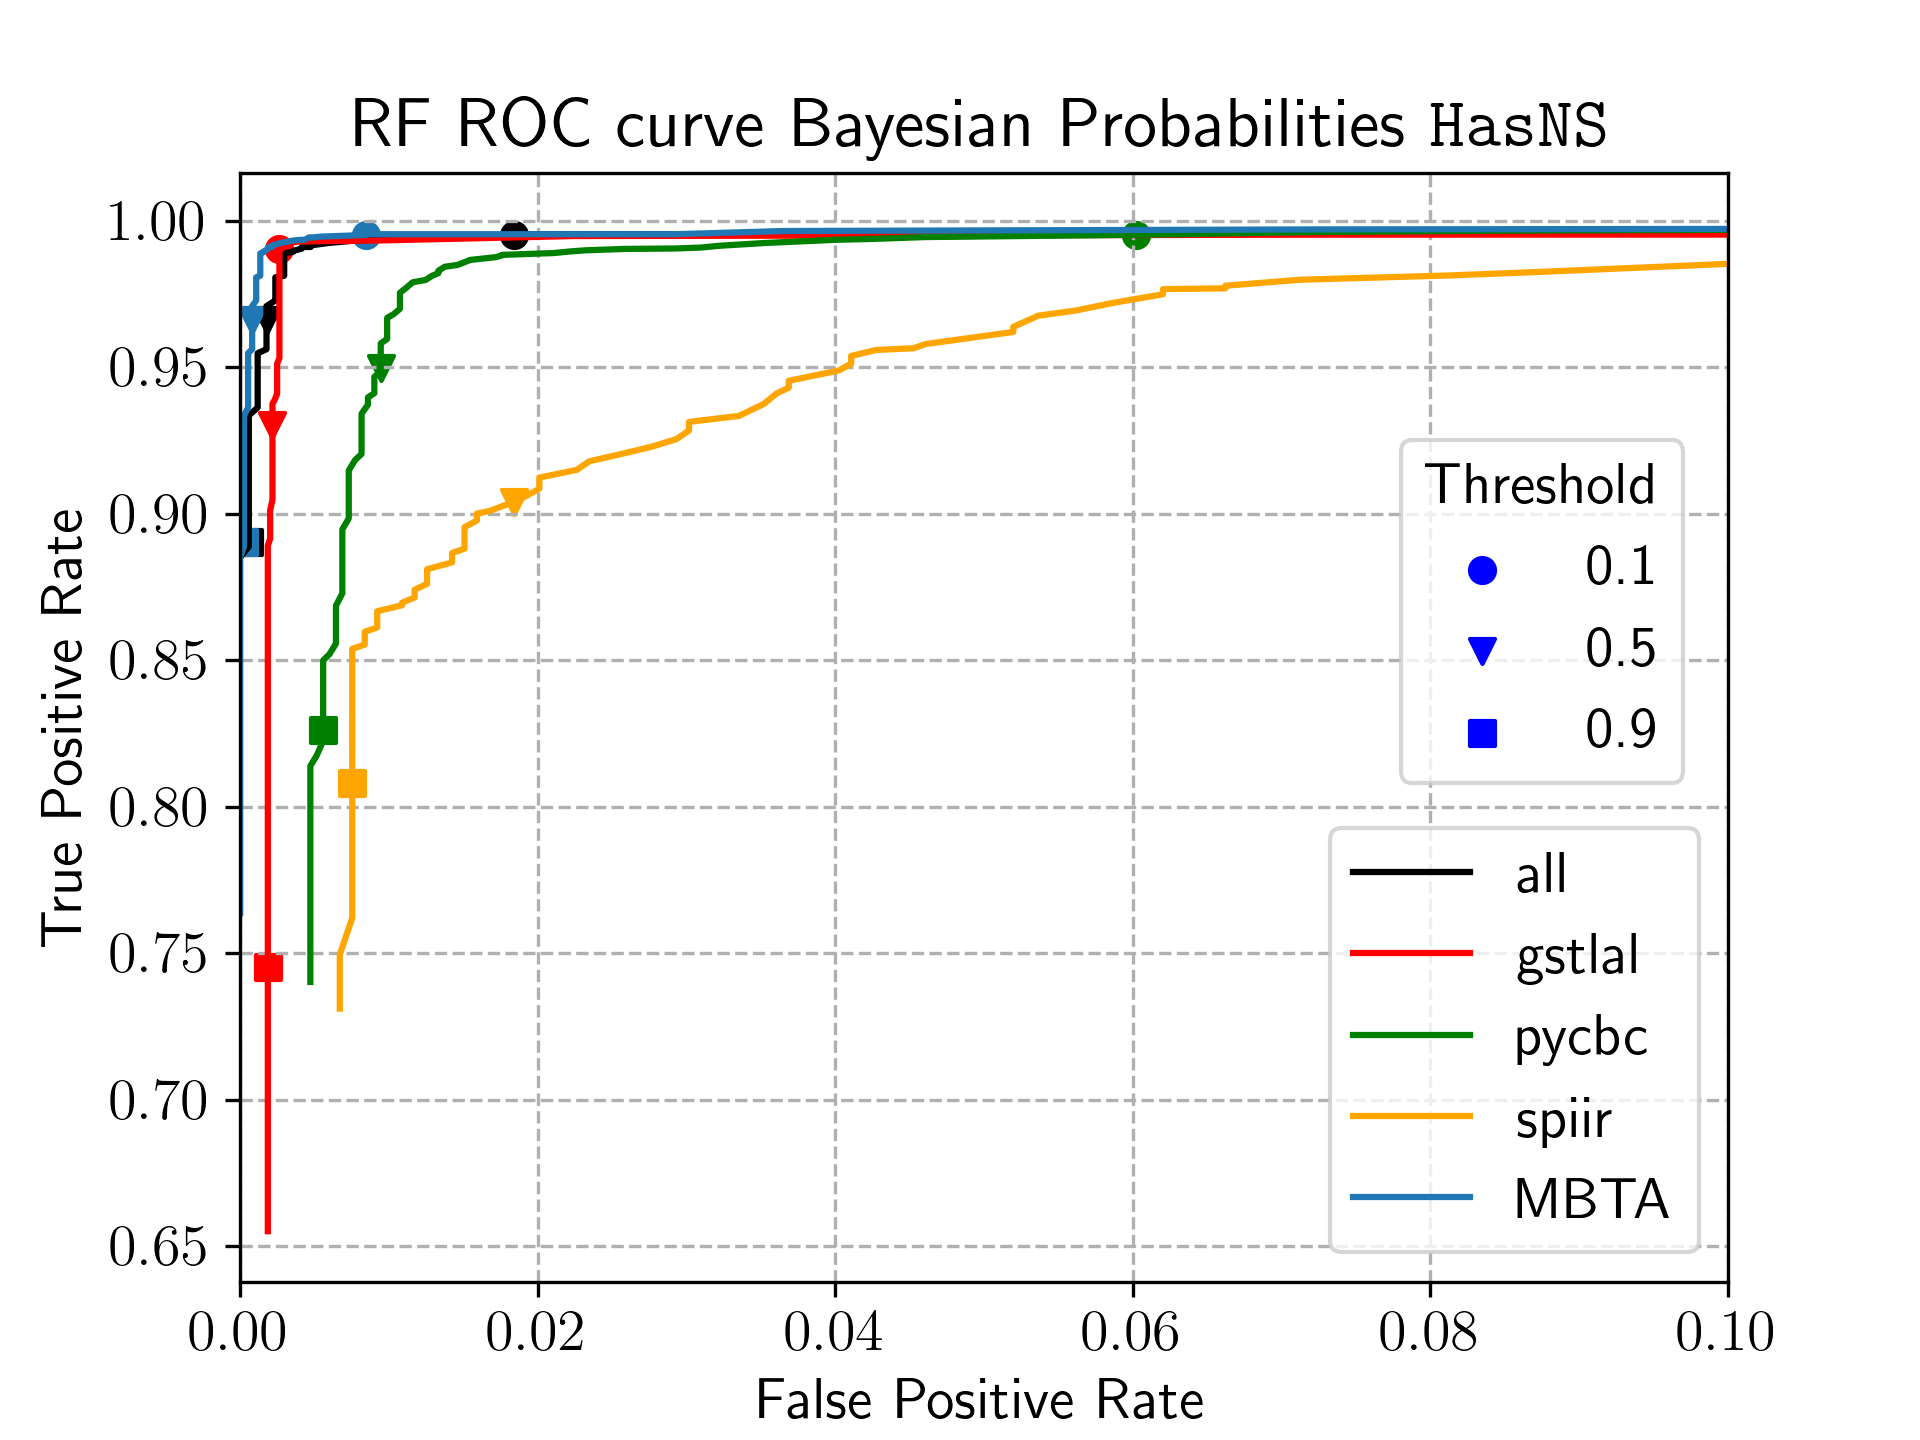
\includegraphics[width=0.45\linewidth]{RF_bayesian_NS}
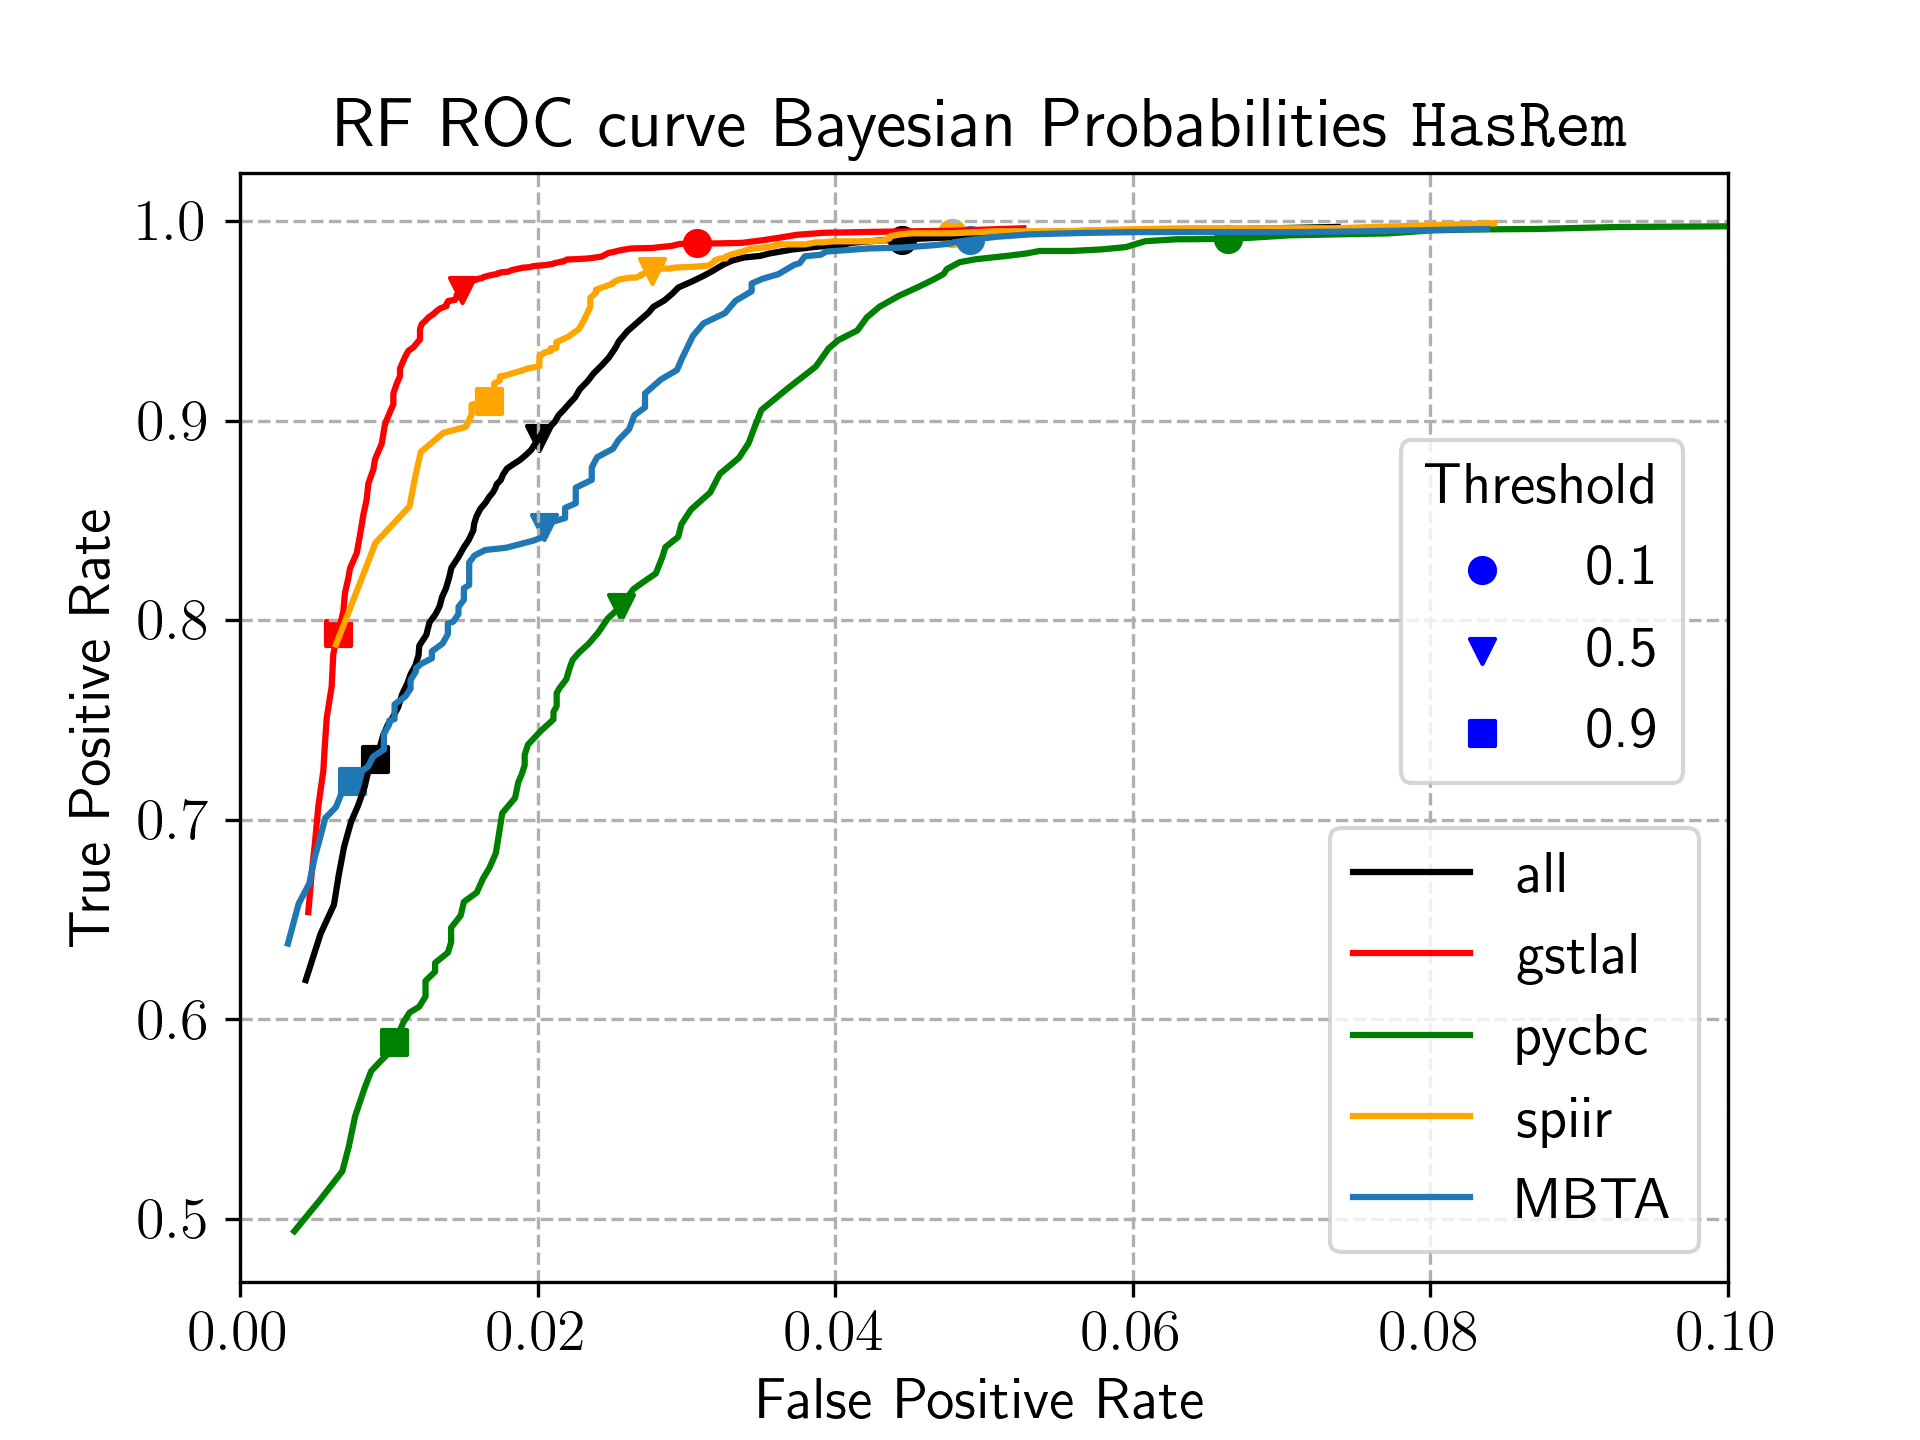
\includegraphics[width=0.45\linewidth]{RF_bayesian_REM}
\caption{ROC curves of Bayesian probability marginalized for the 23 EoSs for MDC11 dataset using \ac{RF} classifier.}
\label{fig:rocMDC_RF}
\end{figure*}

We also applied the tabulated Bayesian probabilities to classify real events
from the O3 LVK run~\cite{LIGOScientific:2020ibl, LIGOScientific:2021djp}.  In Table~\ref{tab:real_data_bayesian} we depict some of the most significant events of the LVK third observing run, labeling them with their event ID and the GraceDB\footnote{\href{https://gracedb.ligo.org/}https://gracedb.ligo.org/} ID.  We show the marginalized Bayesian probabilities for both \hasns\ and \hasrem\ computed with 
\ac{RF} and \ac{KNN}. For the first two events (GW170817 and GW190425),
$P_M(\hasns)$ and $P_M(\hasrem)$ are very close to 1, meaning that these events
correspond to BNS mergers, as shown in~\cite{LIGOScientific:2020ibl,LIGOScientific:2021djp}. 
For GW190426 and GW200115, $P_M(\hasns) \sim 1$, but
$P_M(\hasrem) = 0$, which correspond to NSBH mergers, and agree 
with~\cite{LIGOScientific:2020ibl, LIGOScientific:2021djp}. Finally, GW190814 and GW190924,
have non-zero $P_M(\hasns)$ (indeed, \ac{KNN} gives a probability higher than
0.5 for GW190814). The results in~\cite{LIGOScientific:2020ibl, LIGOScientific:2021djp} show that these events are high mass-ratio BBH mergers. The fact that the component masses are very different from each other (and the lower mass is close to the NS limit) might have led to these non-zero probabilities. 


\begin{table}[]
\begin{tabular}{c|c|cc|cc}
\hline
\multicolumn{1}{c|}{}         & \multicolumn{1}{l|}{} & \multicolumn{2}{c|}{$P_M(\hasns|{\bf A}_{\bf E})$}                                                & \multicolumn{2}{c}{$P_M(\hasrem|{\bf A}_{\bf E})$}                                                \\ \hline
\multicolumn{1}{c|}{event ID} & grace\_id             & \multicolumn{1}{c}{RF} & \multicolumn{1}{c}{KNN}  & \multicolumn{1}{c}{RF} & \multicolumn{1}{c}{KNN} \\ \hline
GW170817                      & G298048               & 0.998                   & 0.989                    & 0.997                   & 0.985                                  \\
GW190425                      & G330564               & 0.998                   & 0.989                    & 0.997                   & 0.985                            \\
GW190426                      & G330687               & 0.997                   & 0.985                    & 0.000                   & 0.000                     \\
GW190814                      & G347305               & 0.042                   & 0.567                   & 0.000                  & 0.000                      \\
GW190924                      & G351423               & 0.012                   & 0.054                   & 0.000               & 0.000                       \\               
GW200115                      & G360364               & 0.998                   & 0.989                   & 0.000                  & 0.000                           \\
\hline
\end{tabular}
\caption{Short table with marginalized BAYESIAN probabilities for O3 real events.}
\label{tab:real_data_bayesian}
\end{table}

In Figs.~\ref{fig:param_sweep_KNN} and~\ref{fig:param_sweep_RF} we depict parameter sweeps that are built using the Bayesian probabilities computed with KNN and RF, respectively.  These figures show the Bayesian probability for \hasns\ (left column) and for \hasrem\ (right column) for given component masses of the binary system, being $m_1$ the larger mass. The  columns stand for different fixed values of the component spins. The SNR is fixed to 10. One can see that both algorithms perform in a similar way. Regarding $P_M(\hasns)$,  there are no notable differences between the choice of spin values.  There is a small difference between the algorithms: for the third column ($\chi_1 = 0.0$ and $\chi_2$), $P_M(\hasns)$ is larger for bigger $m_1$ in the case of KNN.   For $P_M(\hasrem)$, both algorithms give almost the same results. The sweeps show that, for a large $\chi_1$, the probability of having a remnant increases for bigger values of the first component mass, $m_1$. As expected, the region in which $P_M(\hasrem) \sim 1$ is inside the region in which $P_M(\hasns) \sim 1$.

Moreover, the Bayesian probabilities seem to be more uniform for RF in all the cases, and KNN gives some blobs of larger probability \mmt{[MMT: I don't know how to explain this]}.

\begin{figure*}%[h]
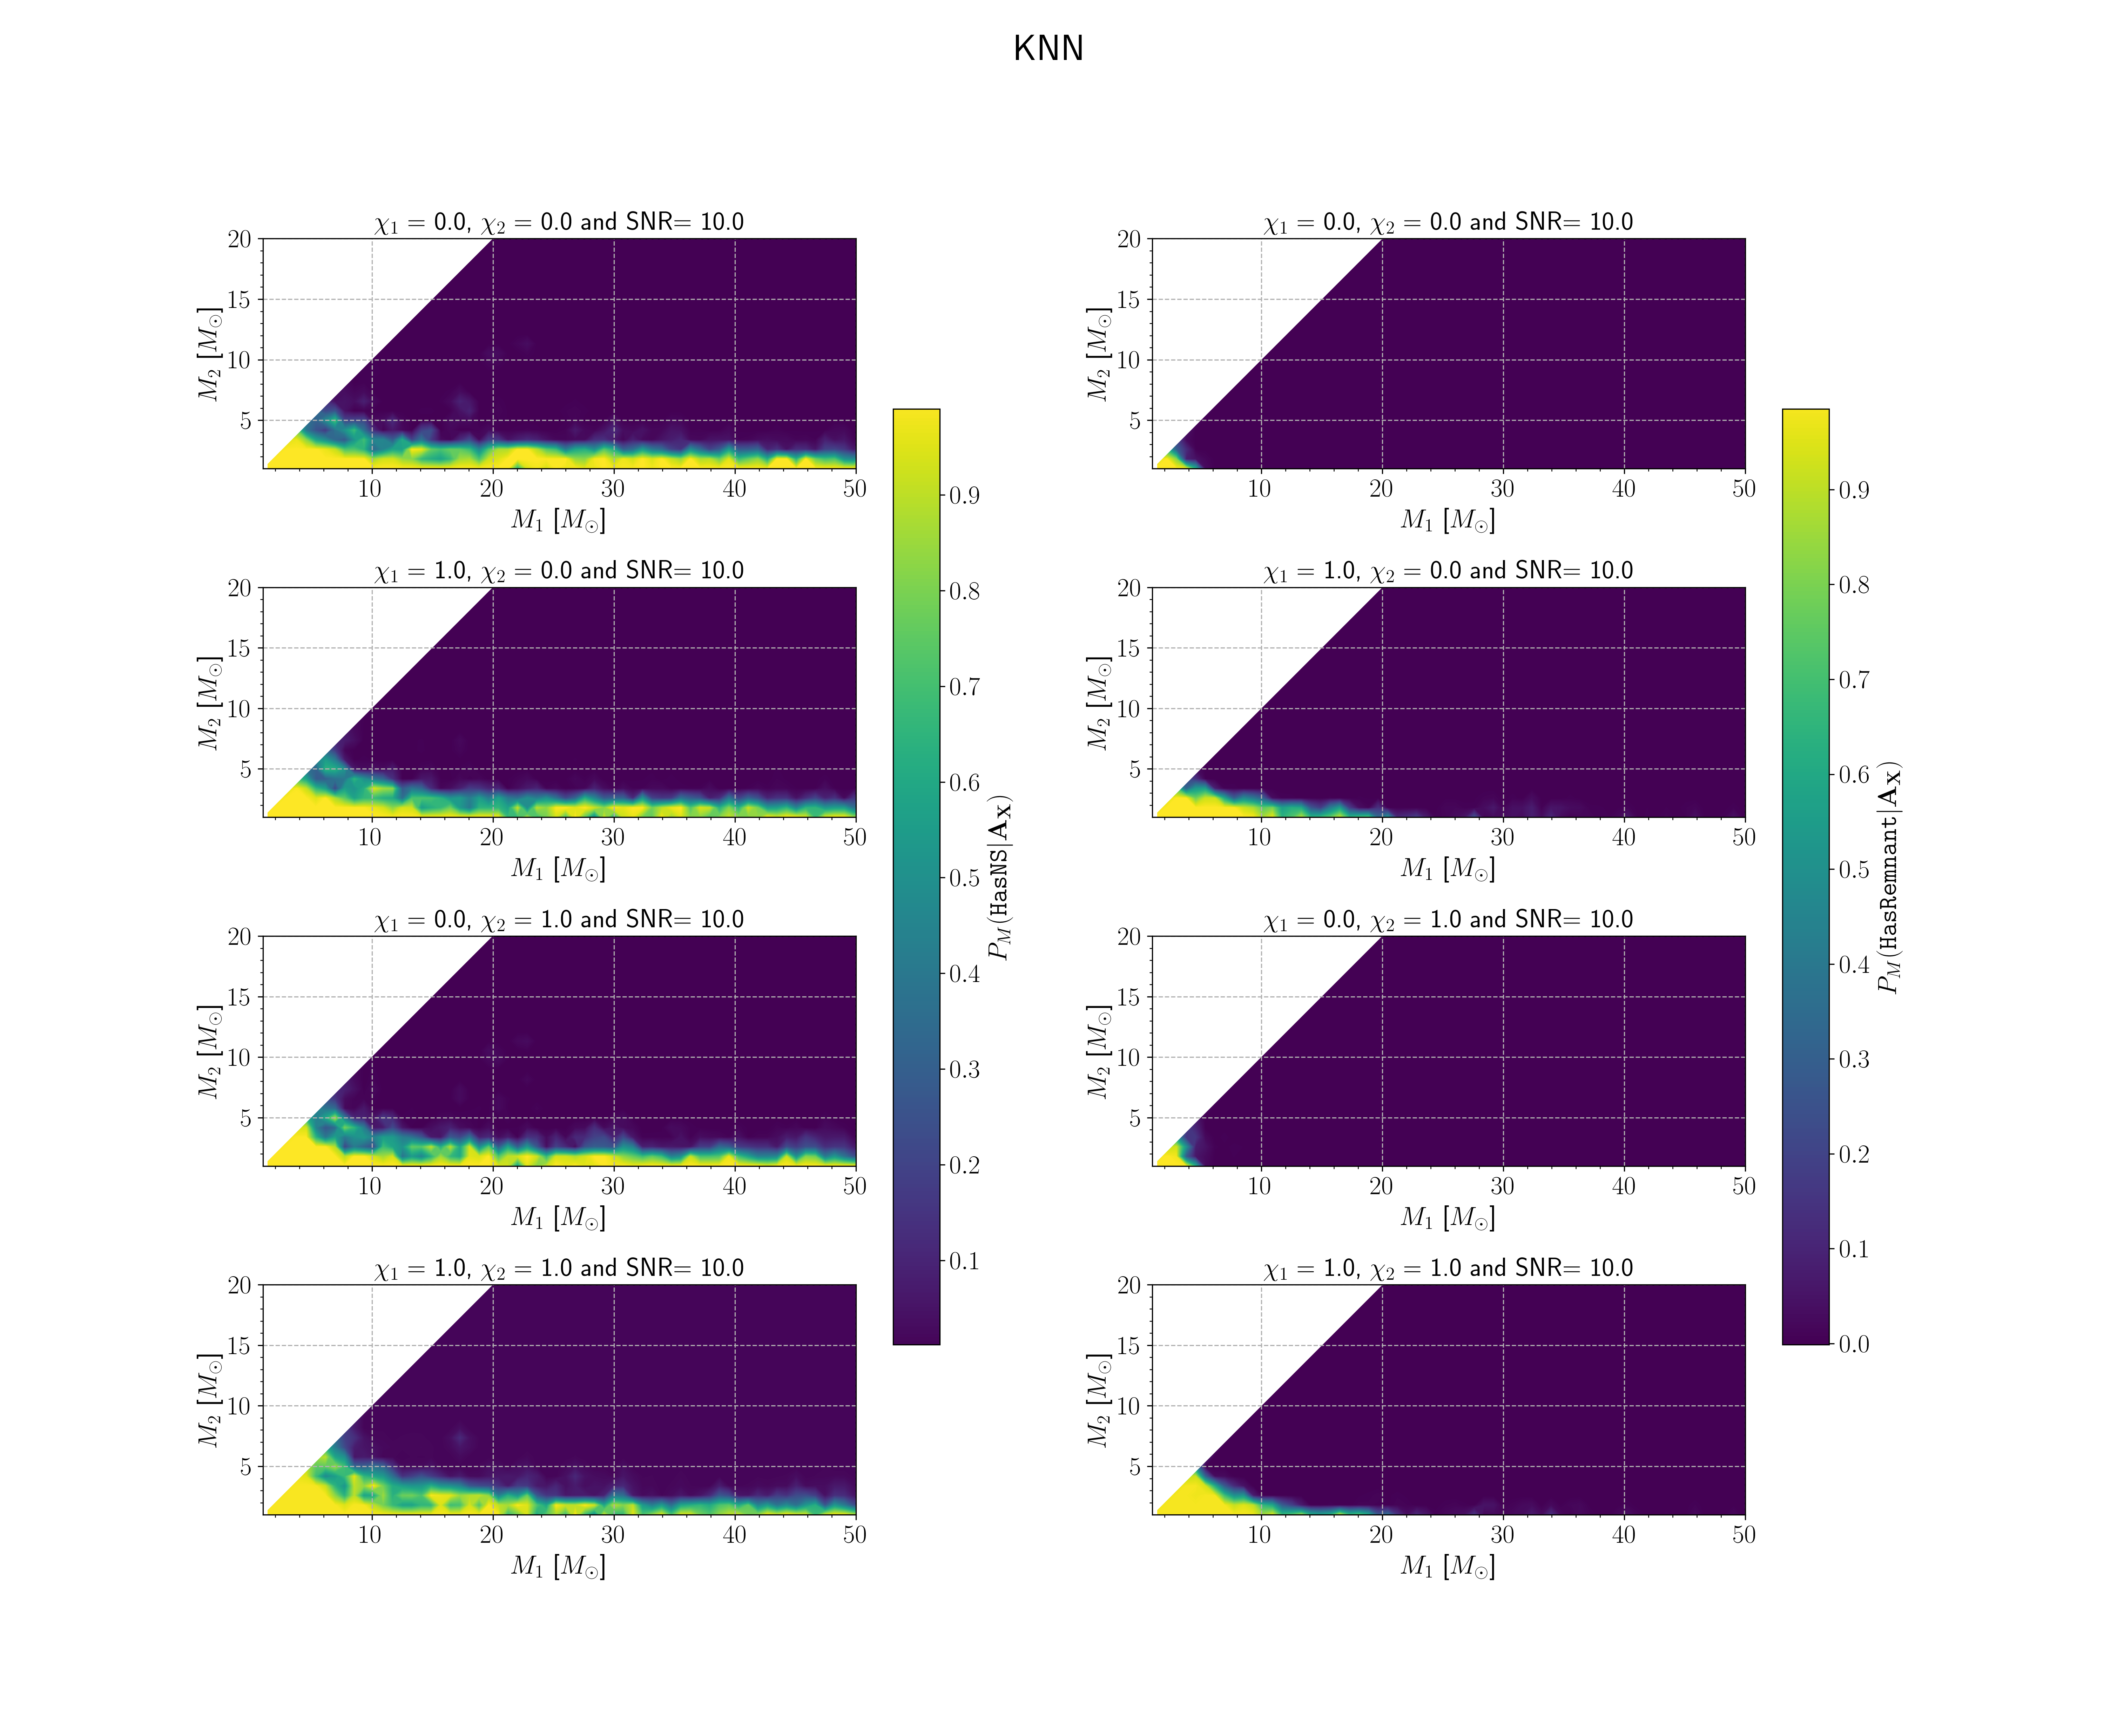
\includegraphics[width=0.7\linewidth]{KNN_parameter_sweep}
    \caption{Parameter sweep obtained with KNN. The Bayesian probabilities are shown as a function of the component masses of the binary, where $m_1$ (the bigger mass) is in the horizontal axes and $m_2$, in the vertical. The left panels show $P_M(\hasns)$ and the right panels, $P_M(\hasrem)$. We choose different values of the spin components to evaluate the probability, and they appear in the different rows of the figure.   The SNR is fixed to 10. }
\label{fig:param_sweep_KNN}
\end{figure*}

\begin{figure*}%[h]
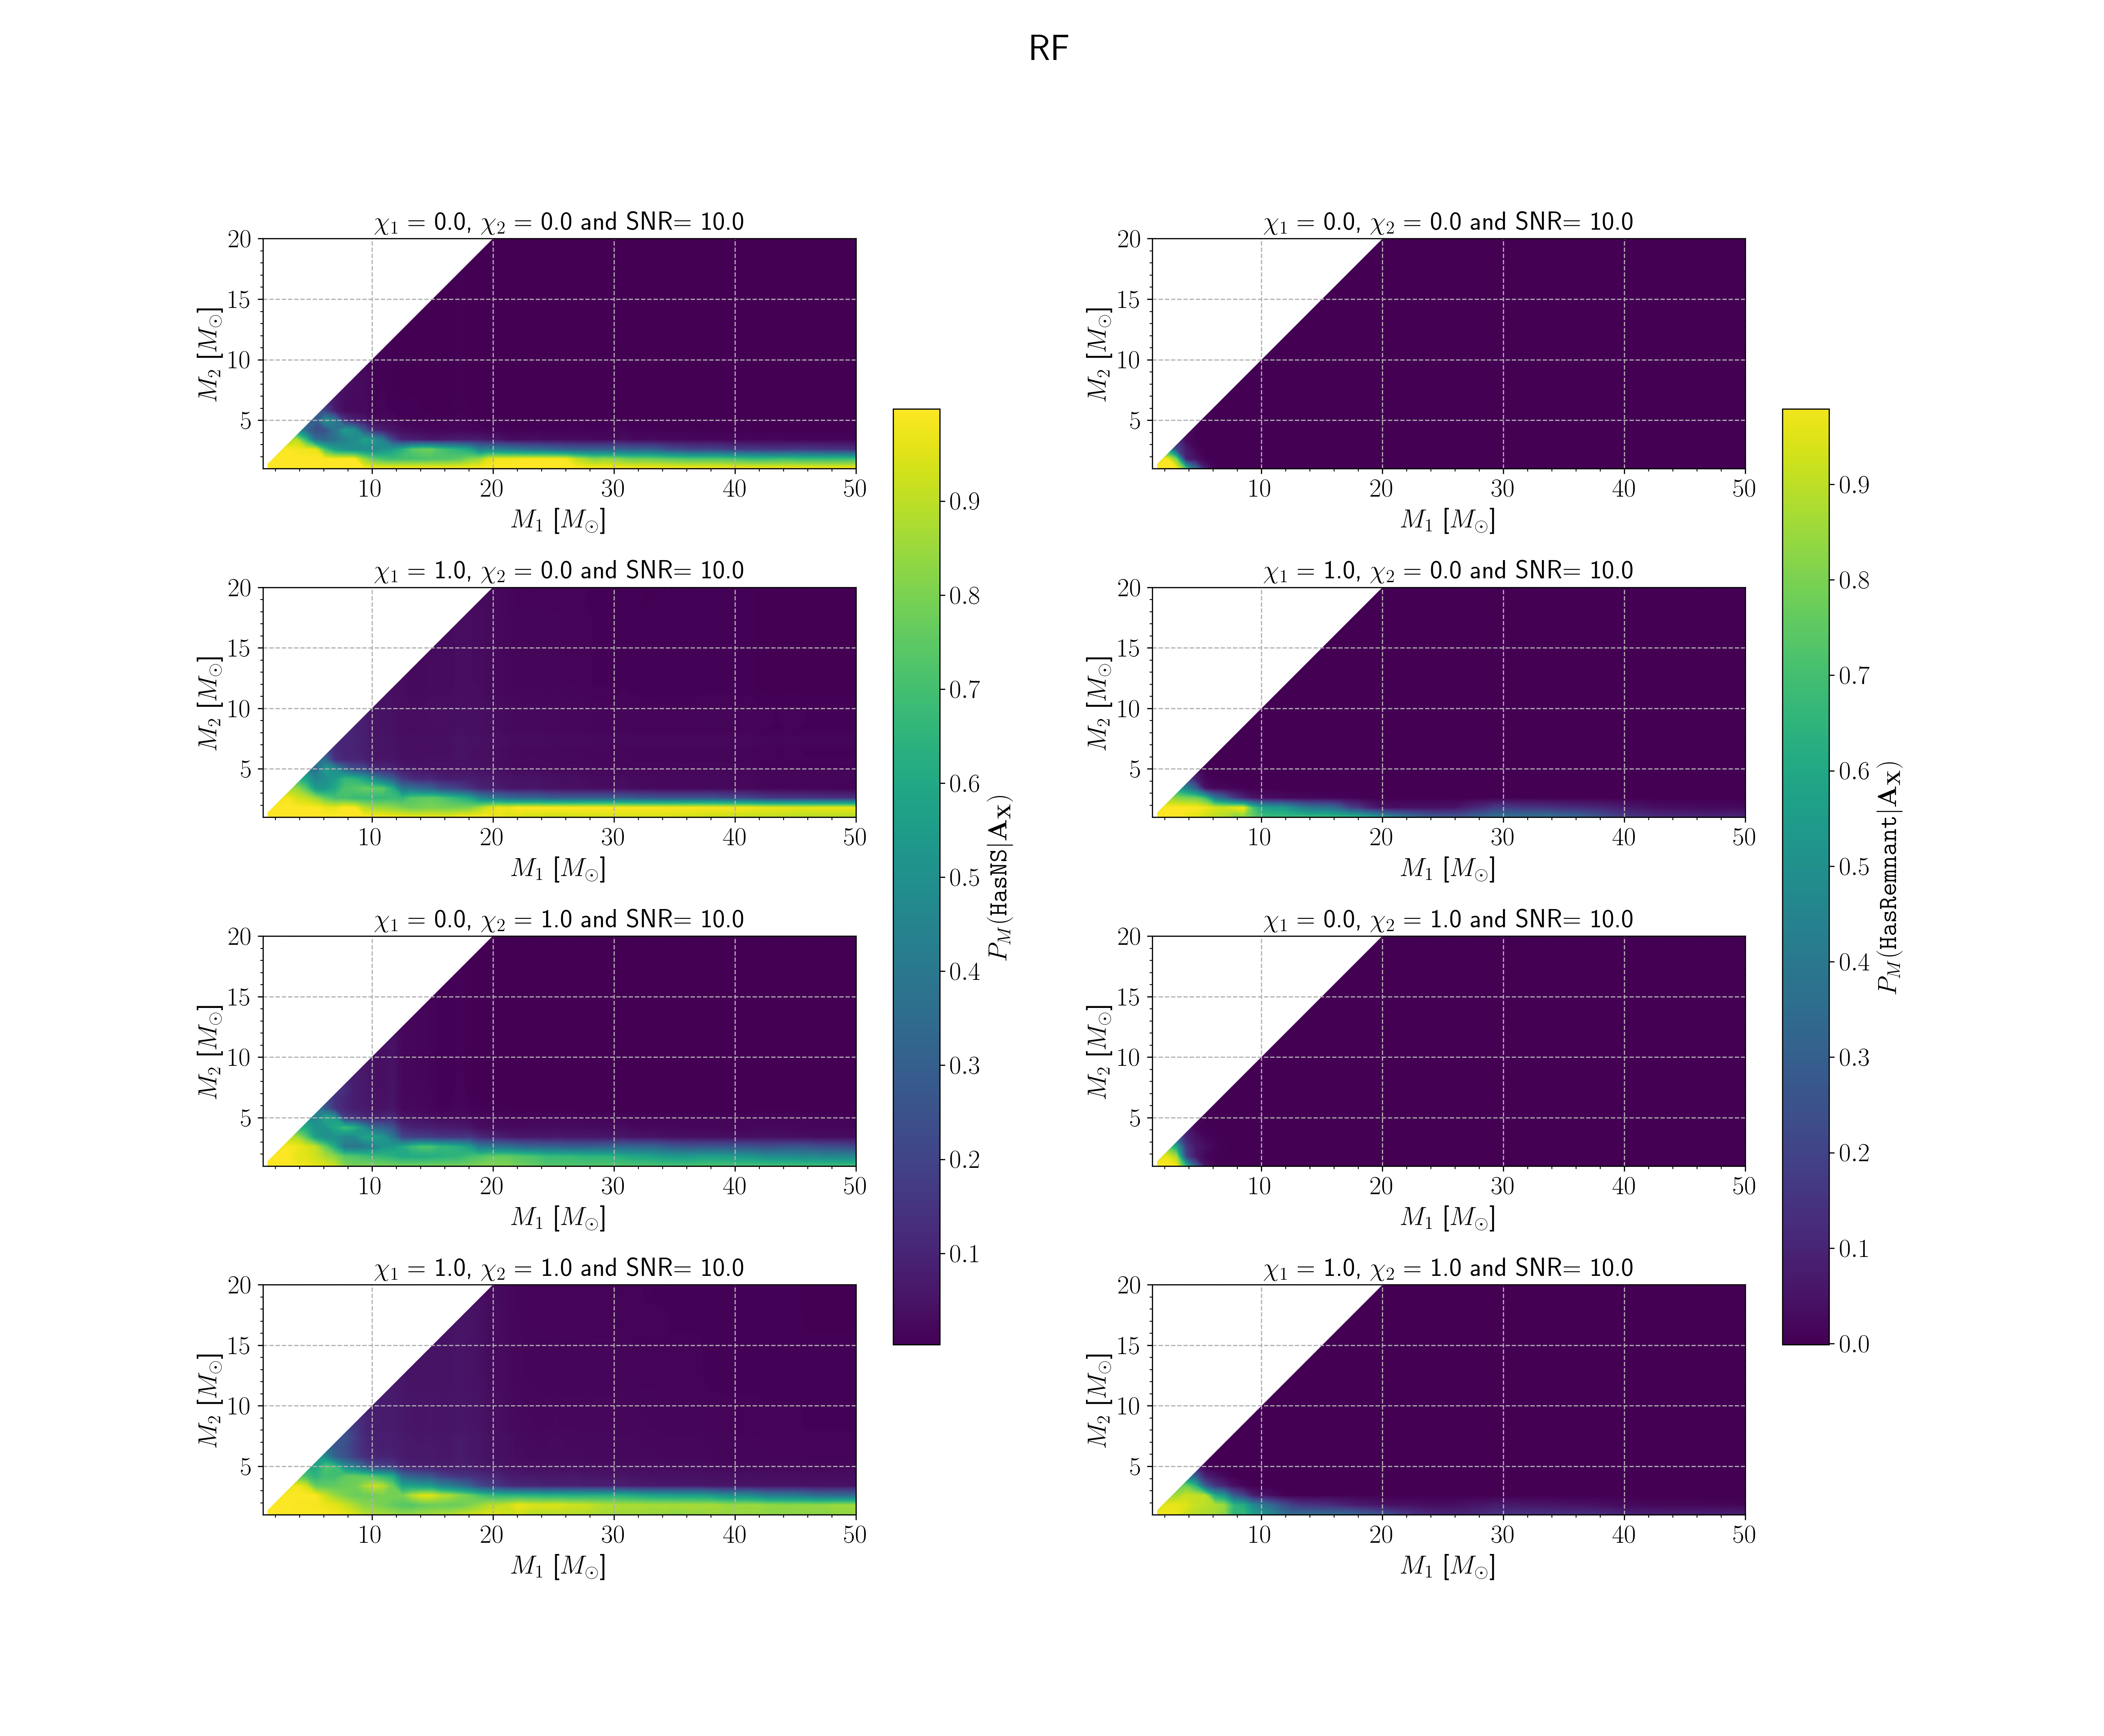
\includegraphics[width=0.7\linewidth]{RF_parameter_sweep}
 \caption{Same as Figure~\ref{fig:param_sweep_KNN}, but now for RF.}
\label{fig:param_sweep_RF}
\end{figure*}


%Here are the results for the methods:

%\subsection{KNN Results}

%\mmt{We are only using 5 features, the independent variables: 
%\begin{equation*}
	%\big[m_1,m_2,\chi_1,\chi_2, \rm{SNR}\big]\,.
%\end{equation*}}

\subsubsection{\mmt{Has NS}}
\mmt{The metric we use to compute the distance between neighbors is the \textit{Manhattan} metric (or the Minkowski's $L1$ distance),  which is the distance between two points measured along axes at right angles. Having $p_1(x_1,y_1)$ and $p_2(x_2,y_2)$ the distance will be}
\begin{equation}
	d = |x_1-x_2|+|y_1-y_2|\,.
\end{equation}

\mmt{Moreover, the points are weighted uniformly.  After applying cross-validation,  we get that the optimal number of neighbors is $K_{\rm NS} = 10$, with a mean score $\rm{s_m} = 0:9718355224352762$ and a testing score  $\rm{s_t} = 0.9723828730478842$.} 

%\begin{figure}
%    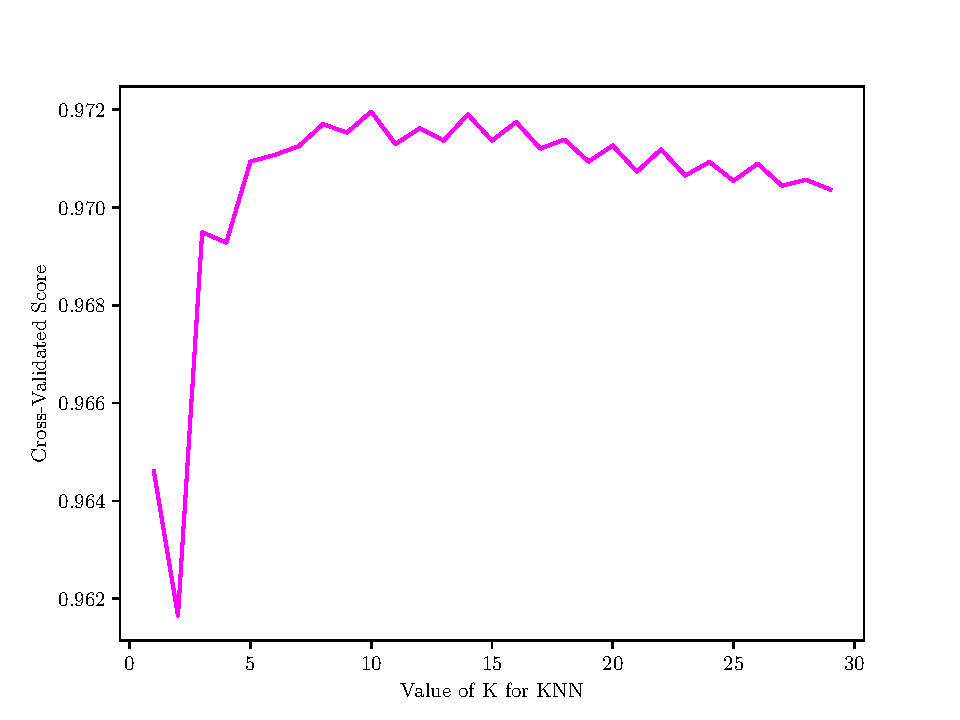
\includegraphics[width = 0.4\textwidth]{CrossValK.pdf}
%    \caption{Score of our KNN model as a function of the number of neighbors. We are considering \textit{HasNS}.}
%    \label{fig:crossvalK}
%\end{figure}
    
\begin{figure}
    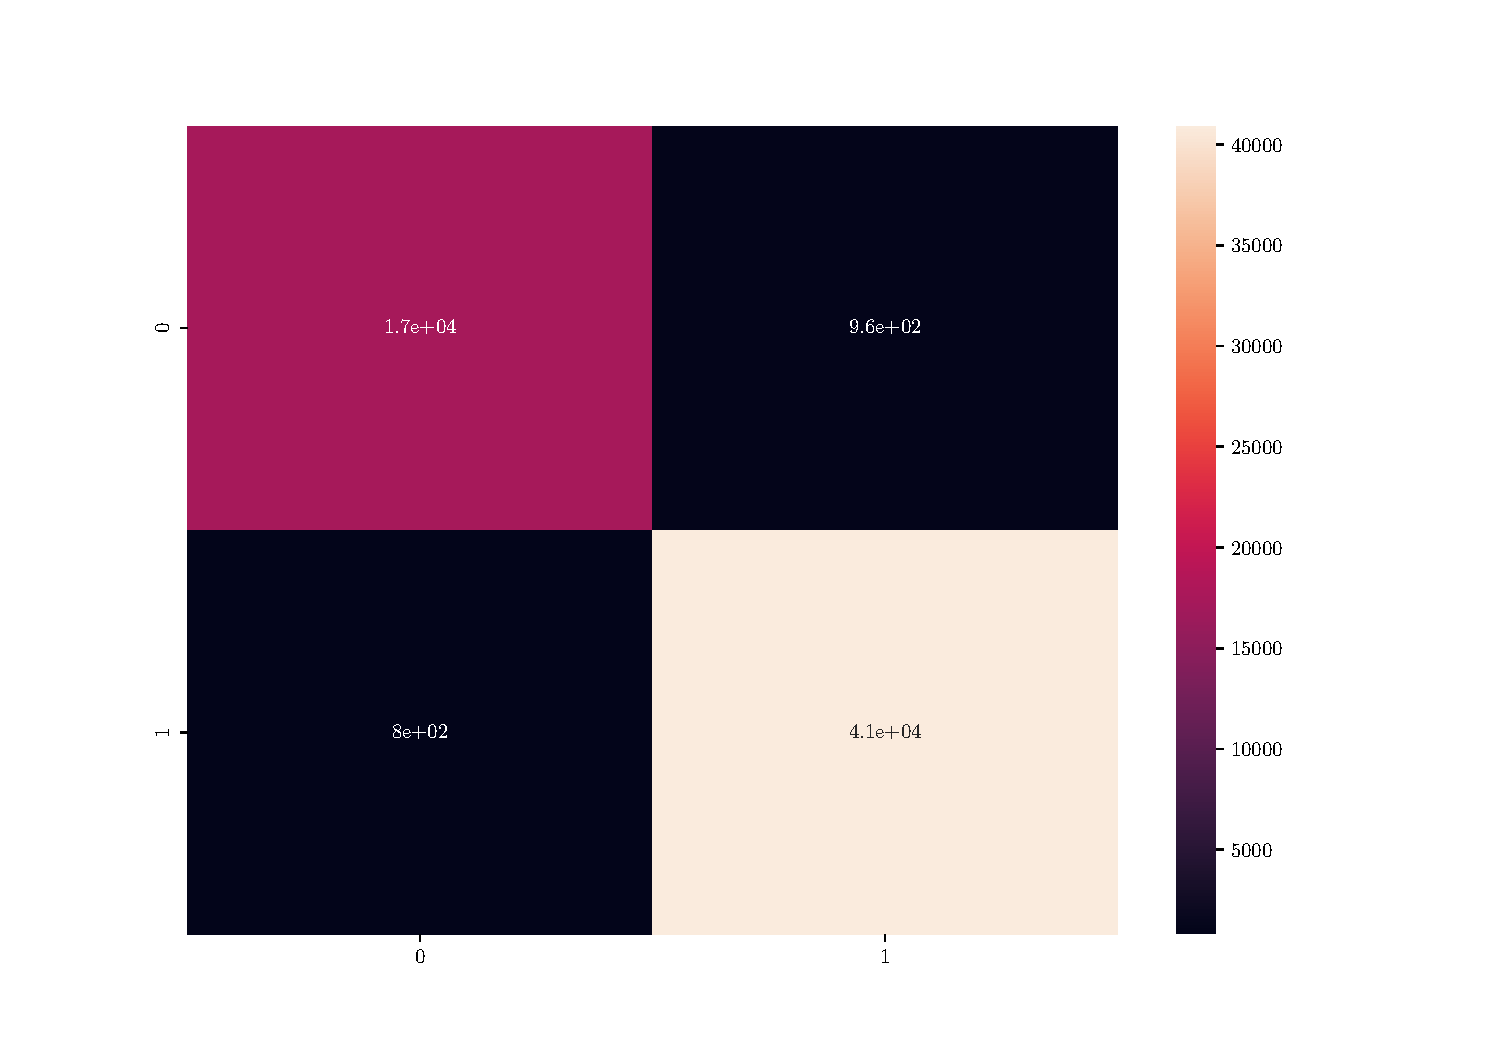
\includegraphics[width=0.45\textwidth]{figs/conf_matrix_NS.pdf}
    \caption{Confusion matrix for our model for \textit{HasNS}, using the independent recovered values. }
    \label{fig:confmat}
\end{figure}

\begin{figure}
    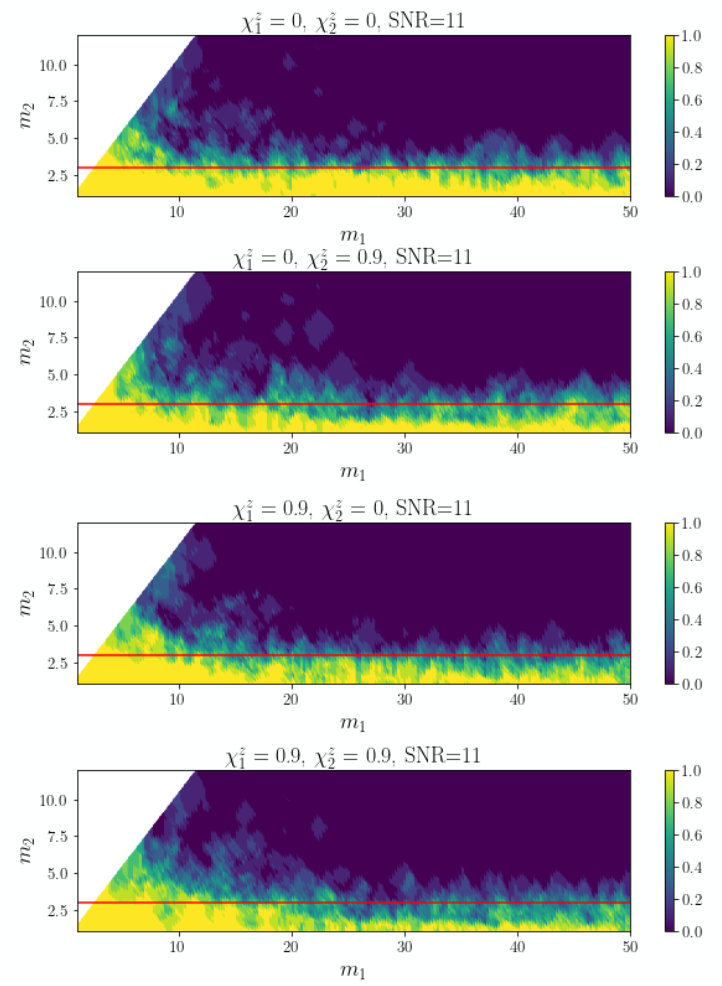
\includegraphics[width = 0.4\textwidth]{plot_fig4_chatt_spins.png}
  %   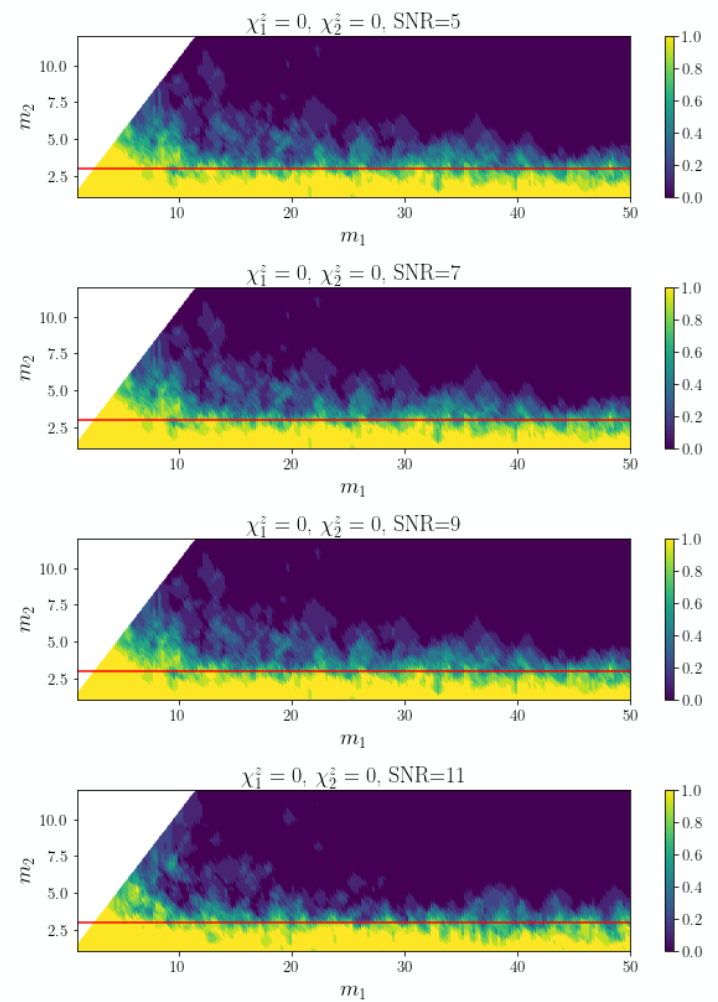
\includegraphics[width = 0.4\textwidth]{/Users/miquelmiravet/Projects/IPAM_LA/ML_group/IPAM2021_ML/algo/classy_KNN/PLOTS_KNN/NS_set/plots_miq/plot_fig4_chatt_snr.png}
    \caption{Probability of having a remnant as a function of the values of the masses. The different panels show the results for different spins. The solid red line depicts the threshold mass for $m_2$.}
    \label{fig:m1m2}
\end{figure}

\begin{figure}
	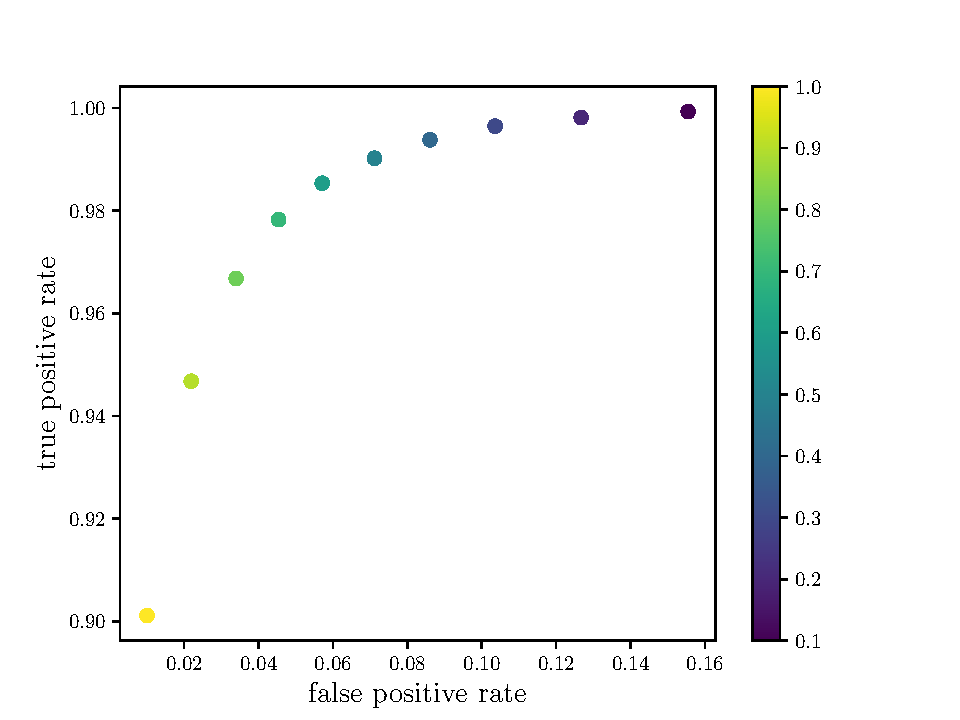
\includegraphics[width =0.4\textwidth]{ROCplot.pdf}
    \caption{Relation of the true and false positive rates as a function of the threshold applied to make the decision between having or not having a remnant. }
    \label{fig:roc}
\end{figure}

\mmt{In Fig.~\ref{fig:crossvalK} you can find how the mean score changes with the number of neighbors of the algorithm.  The confusion matrix appears in Fig.~\ref{fig:confmat}, the probability as a function of $m_1$ and $m_2$  is shown in Figs.~\ref{fig:m1m2}, and the true and false positive rates in terms of the threshold probability appear in Fig.~\ref{fig:roc}.}


 %plots and comments
%\subsection{RF Results}

We apply crossvalidation in the number of trees and depth of the forests for the 23 EoS, fixing the information gain criteria to \texttt{entropy}. We also save the second best option for comparison, and save both forests for each EoS in order to compare the file size. As the goal is to provide a model that can run in a low latency pipeline the amount of memory it can take is limited, even more when there will be 23 different model for the EoS generalization.

In table \ref{tab:RFcross} we present a summary of best and second best hyperparameters found in the crossvalidation for each EoS, along the memory the model occupies and the difference in the score. As we can see, usually a forest with many trees has a second best option with far less that is lighter in memory and achieves a similar performance. The optimum maximum depth is always 15. Also the score achieved for every EoS is similar, and so we check that our accuracy is not NS model dependent.

\begin{table*}[h]
\centering
\begin{tabular}{@{}lcccccccc@{}}
\toprule
                                & \multicolumn{4}{c}{Best}                                & \multicolumn{4}{c}{Second best}                            \\ \midrule
\multicolumn{1}{|l|}{EOS}       & Trees & Depth & Size(MB)    & \multicolumn{1}{c|}{Score}      & Trees & Depth & Size(MB)    & \multicolumn{1}{c|}{$\Delta$score} \\ \midrule
\multicolumn{1}{|l|}{APR4\_BB}  & 300   & 15    & 94.7  & \multicolumn{1}{c|}{0.9683018}  & 50    & 15    & 15.7  & \multicolumn{1}{c|}{3.35e-5}       \\ \midrule
\multicolumn{1}{|l|}{BHF\_BBB2} & 80    & 15    & 24.4  & \multicolumn{1}{c|}{0.9685127}  & 300   & 15    & 91.6  & \multicolumn{1}{c|}{5.16e-5}       \\ \midrule
\multicolumn{1}{|l|}{H4}        & 80    & 15    & 29.6  & \multicolumn{1}{c|}{0.9618587}  & 300   & 15    & 111.4 & \multicolumn{1}{c|}{1.19e-4}       \\ \midrule
\multicolumn{1}{|l|}{HQC18}     & 300   & 15    & 93.7  & \multicolumn{1}{c|}{0.9673755}  & 100   & 15    & 31.3  & \multicolumn{1}{c|}{3.06e-4}       \\ \midrule
\multicolumn{1}{|l|}{KDE0V}     & 300   & 15    & 92.0  & \multicolumn{1}{c|}{0.9673295}  & 80    & 15    & 24.5  & \multicolumn{1}{c|}{2.06e-4}       \\ \midrule
\multicolumn{1}{|l|}{KDE0V1}    & 100   & 15    & 30.9  & \multicolumn{1}{c|}{0.96704954} & 80    & 15    & 24.5  & \multicolumn{1}{c|}{3.43e-5}       \\ \midrule
\multicolumn{1}{|l|}{MPA1}      & 80    & 15    & 27.2  & \multicolumn{1}{c|}{0.96601225} & 300   & 15    & 102.1 & \multicolumn{1}{c|}{8.19e-5}       \\ \midrule
\multicolumn{1}{|l|}{MS1\_PP}   & 300   & 15    & 113.5 & \multicolumn{1}{c|}{0.96563534} & 80    & 15    & 30.2  & \multicolumn{1}{c|}{1.15e-4}       \\ \midrule
\multicolumn{1}{|l|}{MS1B\_PP}  & 300   & 15    & 114.2 & \multicolumn{1}{c|}{0.96555340} & 100   & 15    & 38.0  & \multicolumn{1}{c|}{1.97e-4}       \\ \midrule
\multicolumn{1}{|l|}{RS}        & 300   & 15    & 103.8 & \multicolumn{1}{c|}{0.96447350} & 80    & 15    & 27.6  & \multicolumn{1}{c|}{2.36e-4}       \\ \midrule
\multicolumn{1}{|l|}{SK255}     & 300   & 15    & 105.8 & \multicolumn{1}{c|}{0.96472405} & 100   & 15    & 35.5  & \multicolumn{1}{c|}{3.69e-4}       \\ \midrule
\multicolumn{1}{|l|}{SK272}     & 300   & 15    & 109.0 & \multicolumn{1}{c|}{0.96401816} & 100   & 15    & 36.4  & \multicolumn{1}{c|}{1.99e-4}       \\ \midrule
\multicolumn{1}{|l|}{SKI2}      & 50    & 15    & 18.8  & \multicolumn{1}{c|}{0.96242338} & 300   & 15    & 112.8 & \multicolumn{1}{c|}{8.37e-5}       \\ \midrule
\multicolumn{1}{|l|}{SKI3}      & 50    & 15    & 19.0  & \multicolumn{1}{c|}{0.96174537} & 100   & 15    & 38.1  & \multicolumn{1}{c|}{6.62e-5}       \\ \midrule
\multicolumn{1}{|l|}{SKI4}      & 300   & 15    & 100.6 & \multicolumn{1}{c|}{0.96598969} & 30    & 15    & 9.8   & \multicolumn{1}{c|}{8.37e-5}       \\ \midrule
\multicolumn{1}{|l|}{SKI5}      & 100   & 15    & 38.2  & \multicolumn{1}{c|}{0.96343381} & 80    & 15    & 30.4  & \multicolumn{1}{c|}{1.16e-4}       \\ \midrule
\multicolumn{1}{|l|}{SKI6}      & 300   & 15    & 101.7 & \multicolumn{1}{c|}{0.96586928} & 30    & 15    & 10.0  & \multicolumn{1}{c|}{2.17e-4}       \\ \midrule
\multicolumn{1}{|l|}{SKMP}      & 300   & 15    & 100.2 & \multicolumn{1}{c|}{0.96544567} & 80    & 15    & 26.9  & \multicolumn{1}{c|}{1.69e-4}       \\ \midrule
\multicolumn{1}{|l|}{SKOP}      & 100   & 15    & 32.3  & \multicolumn{1}{c|}{0.96610459} & 300   & 15    & 96.2  & \multicolumn{1}{c|}{6.85e-5}       \\ \midrule
\multicolumn{1}{|l|}{SLy}       & 80    & 15    & 25.3  & \multicolumn{1}{c|}{0.96728884} & 300   & 15    & 95.2  & \multicolumn{1}{c|}{8.49e-5}       \\ \midrule
\multicolumn{1}{|l|}{SLY2}      & 100   & 15    & 31.8  & \multicolumn{1}{c|}{0.96745868} & 80    & 15    & 25.4  & \multicolumn{1}{c|}{2.38e-4}       \\ \midrule
\multicolumn{1}{|l|}{SLY9}      & 300   & 15    & 101.6 & \multicolumn{1}{c|}{0.96605993} & 100   & 15    & 34.1  & \multicolumn{1}{c|}{1.51e-4}       \\ \midrule
SLY230A                         & 300   & 15    & 95.5  & 0.96714915                      & 100   & 15    & 31.9  & 2.53e-4                            \\ \bottomrule
\end{tabular}
\caption{Comparison of the best and second best RF models obtained during crossvalidation for all EoS. We show the file size in MB of the forest, and the difference in score between the two options.}
\label{tab:RFcross}
\end{table*}

To simplify the model and according to the results of crossvalidation, we train the final forests for all EoS with 50 trees and 15 maximum depth. In figure \ref{fig:RF_roc} we show the ROC curves for all models to give an idea of the performance. Notice that HasREM performs better than HasNS. The ourperformance of HasREM against HasNS in RF is even more noticeable in the histograms in figures \ref{fig:RF_hist_BHFBBB2}, \ref{fig:RF_hist_SLY} and \ref{fig:RF_hist_MS1PP} for the highlighted EoS, where the bars of asigned probabilities do not intersect each other and therefore there exists a threshold value for perfect classification in the testing dataset.

\begin{figure}
\centering
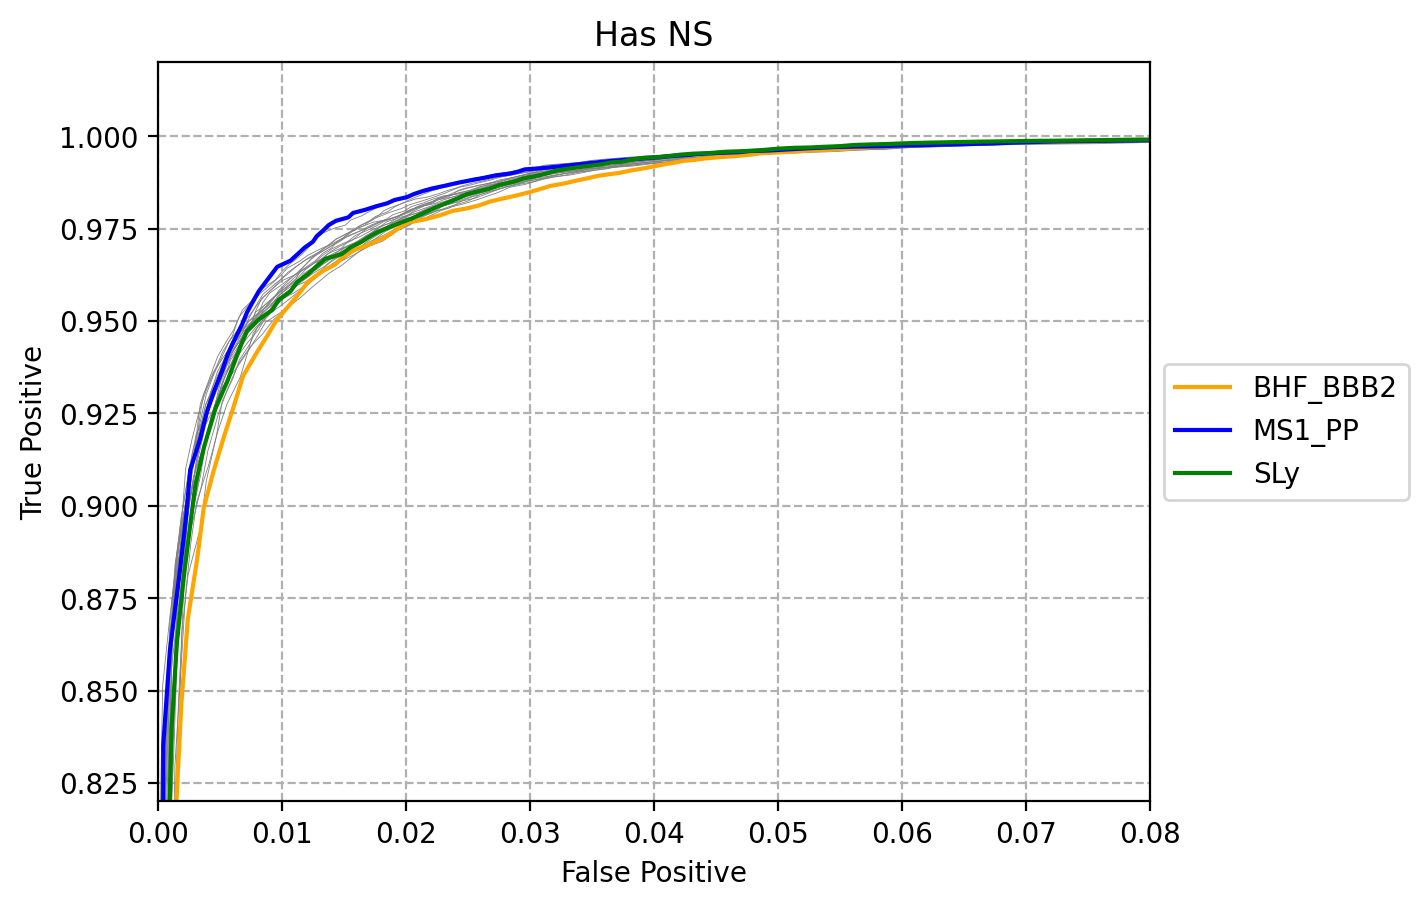
\includegraphics[width=0.45\textwidth]{/figs/HasNS_roc}
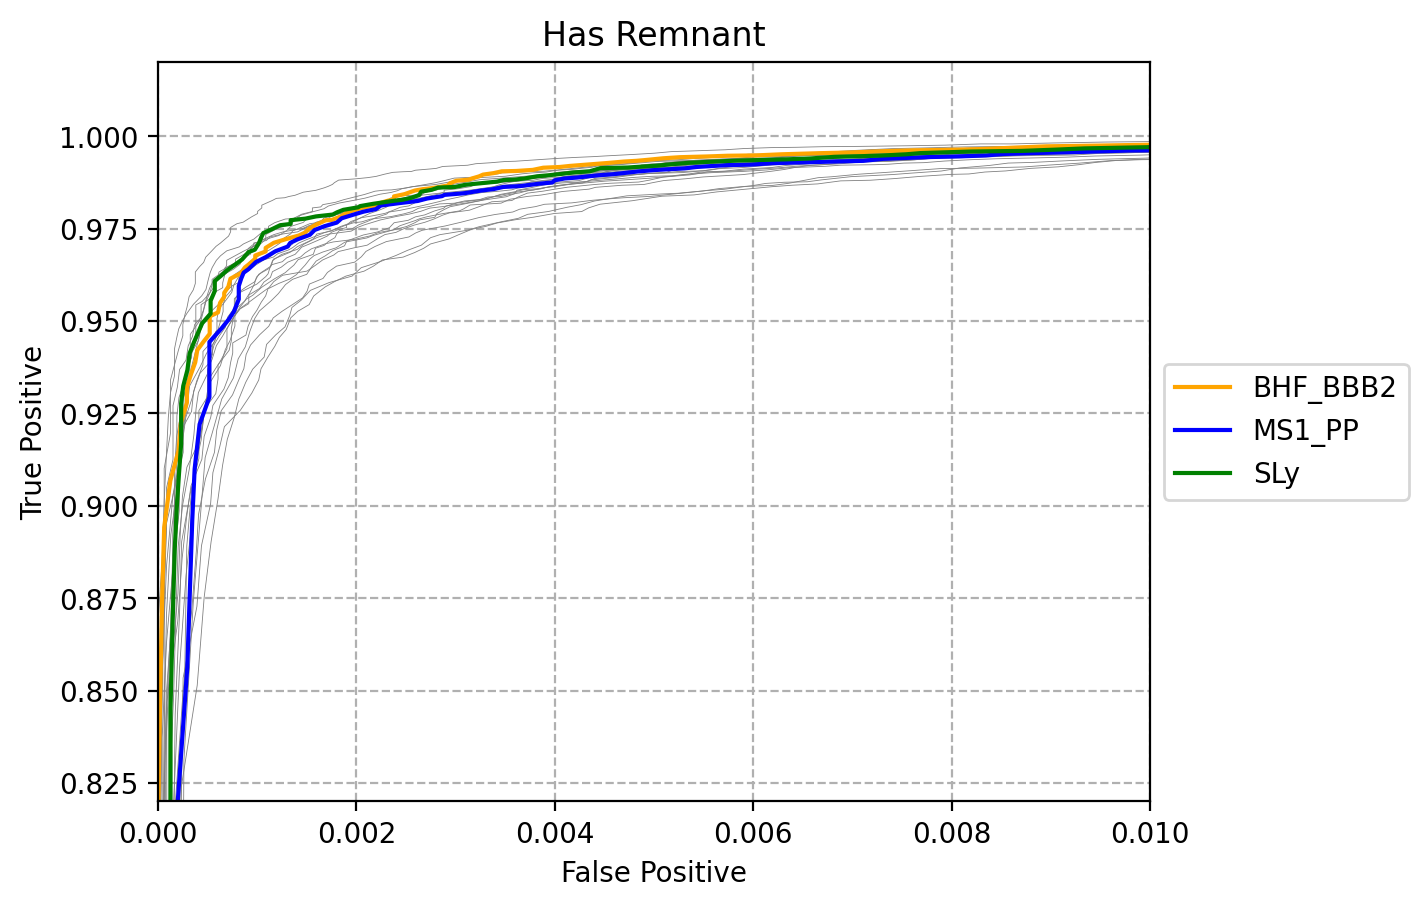
\includegraphics[width=0.45\textwidth]{/figs/HasREM_roc}
\caption{\label{fig:RF_roc} ROC curves}
\end{figure}

\begin{figure}
\centering
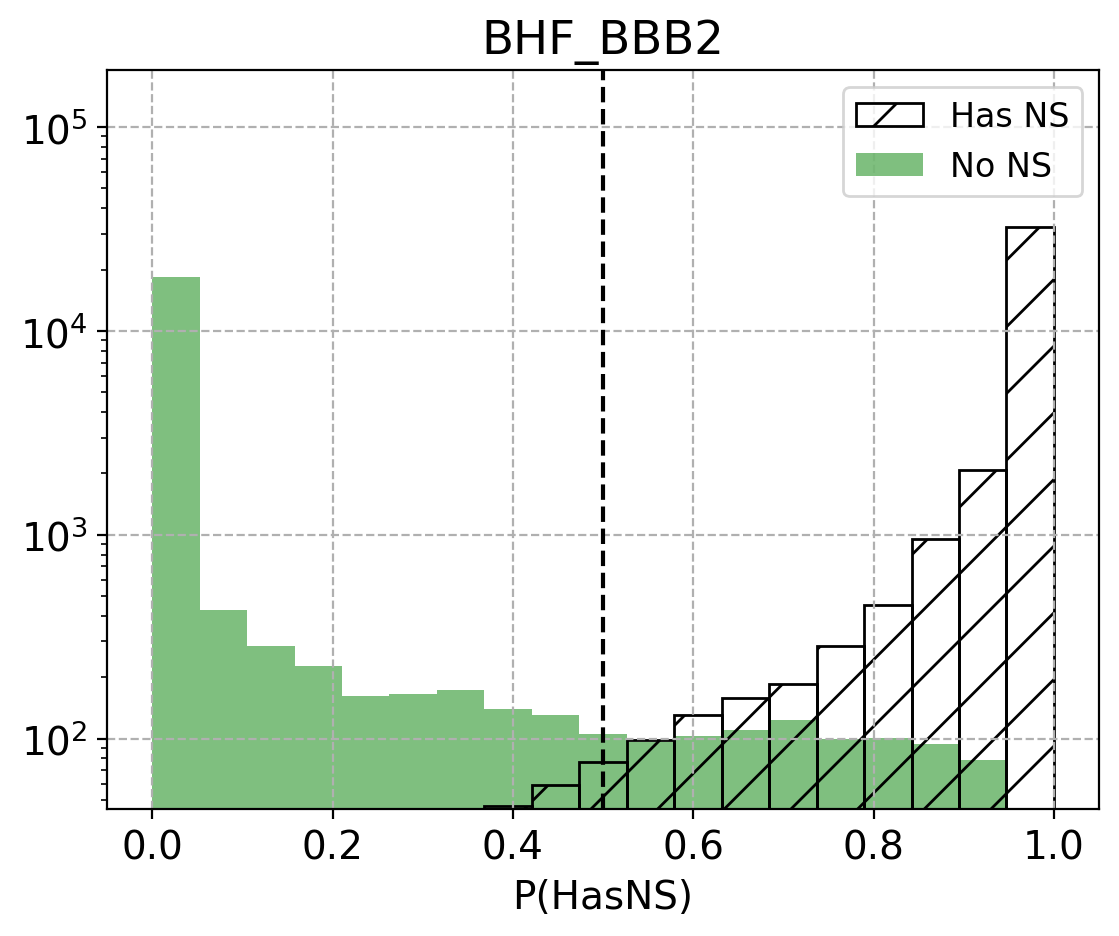
\includegraphics[width=0.45\textwidth]{/figs/BHF_BBB2_NShist}
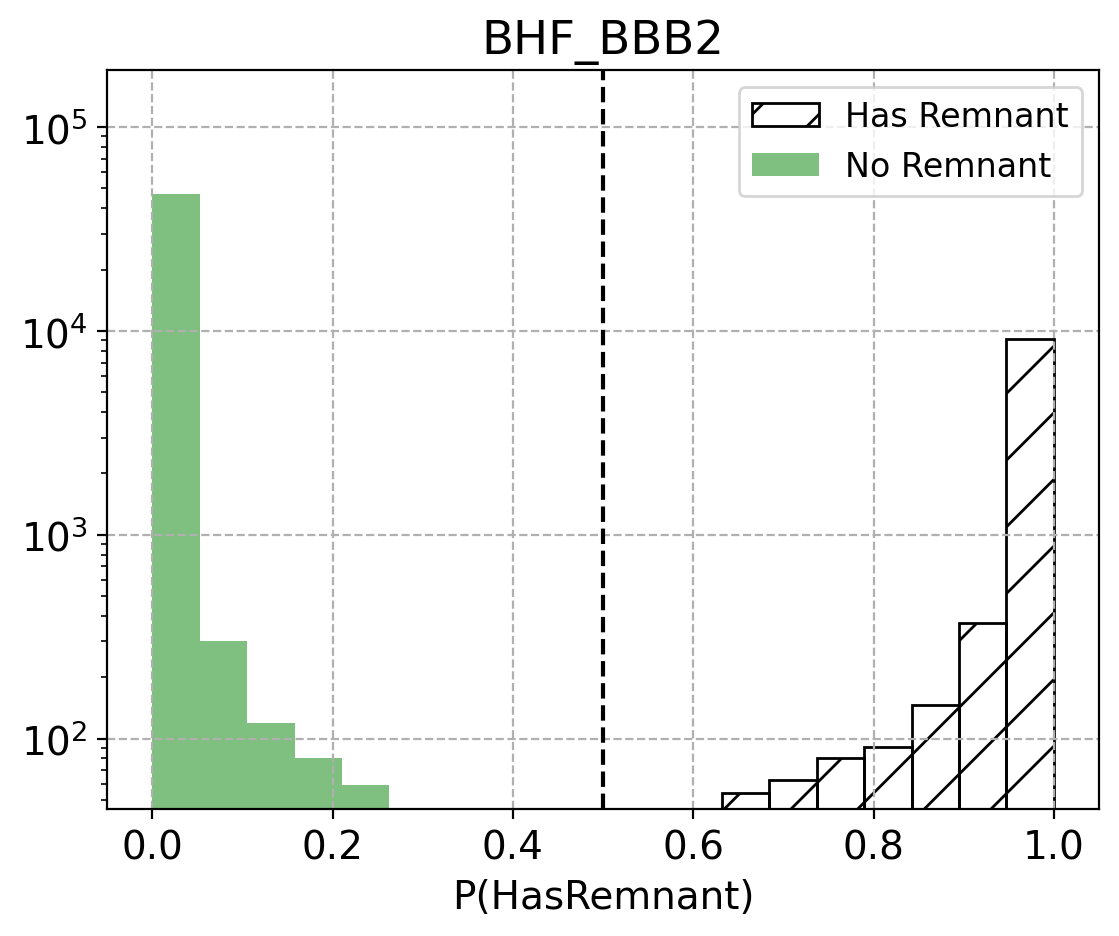
\includegraphics[width=0.45\textwidth]{/figs/BHF_BBB2_REMhist}
\caption{\label{fig:RF_hist_BHFBBB2} Histograms BHF BBB2}
\end{figure}

\begin{figure}
\centering
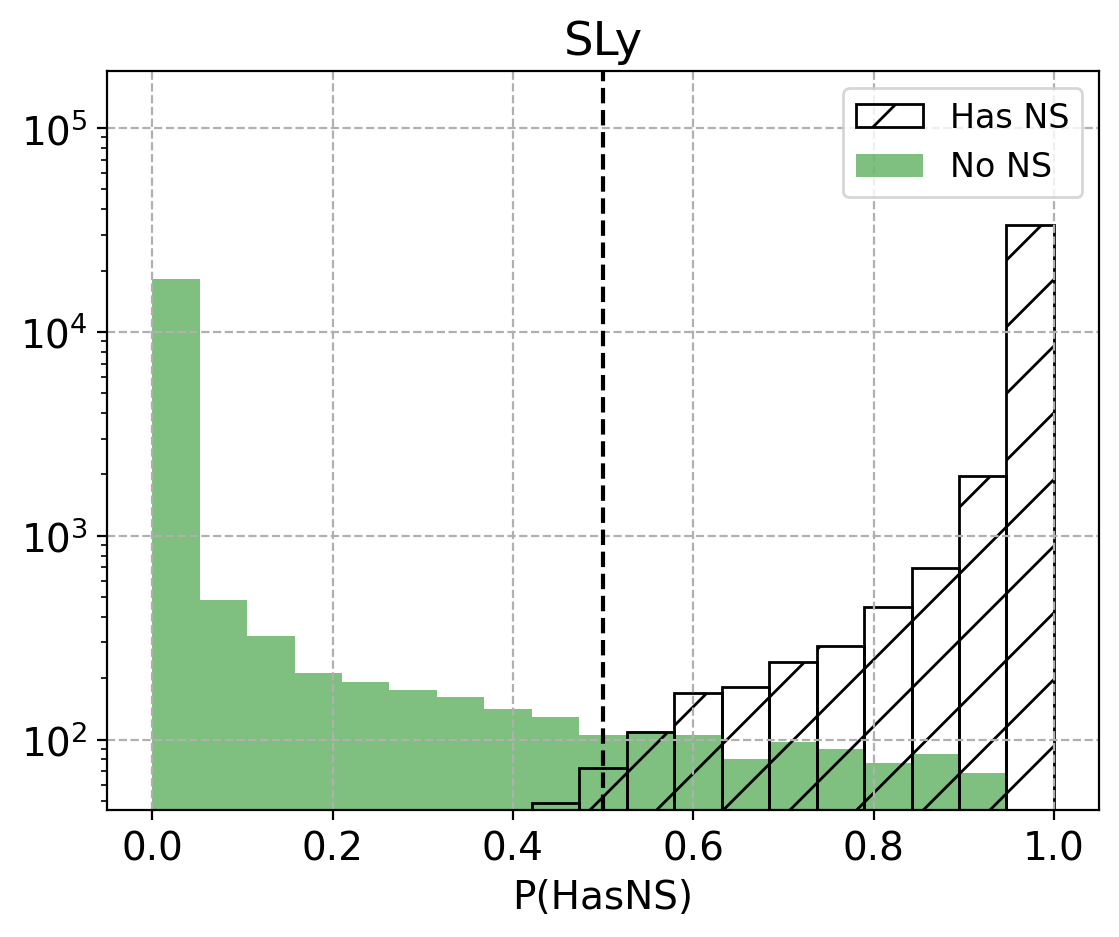
\includegraphics[width=0.45\textwidth]{/figs/SLy_NShist}
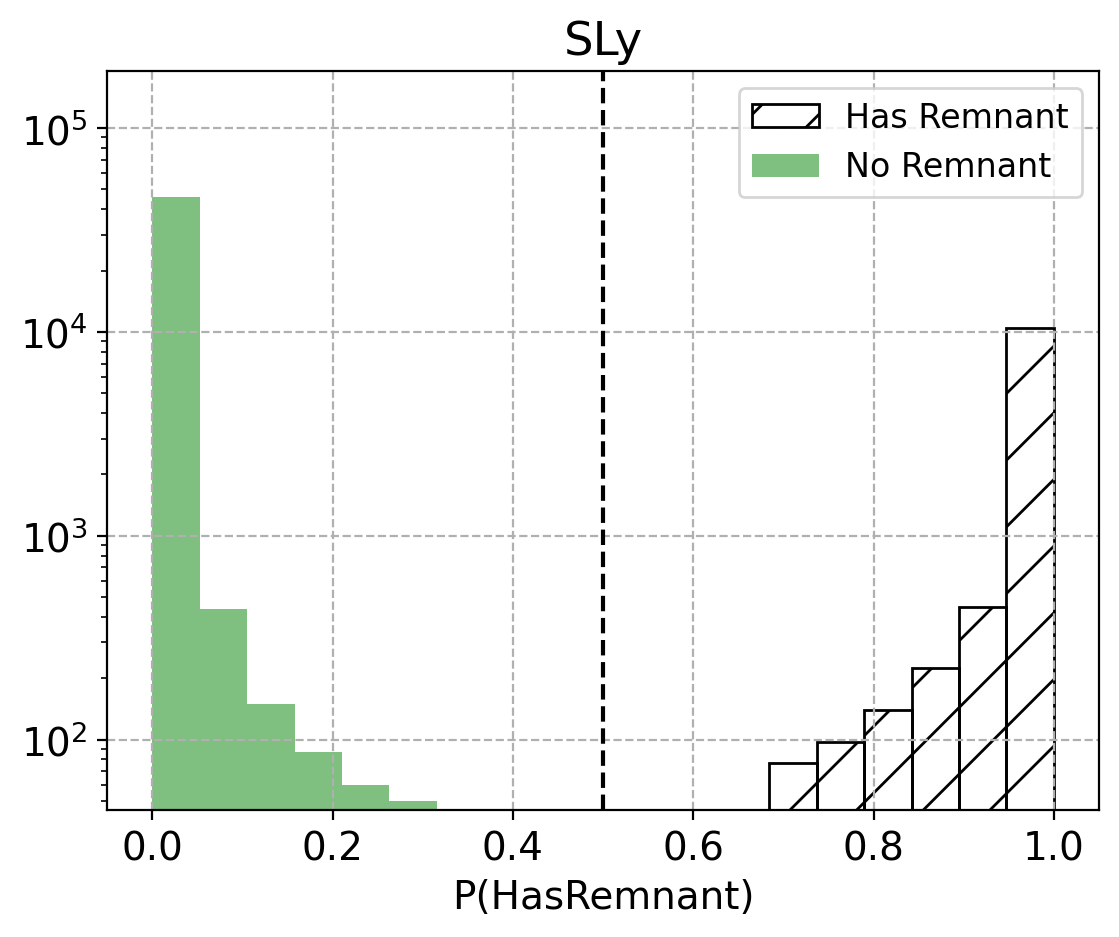
\includegraphics[width=0.45\textwidth]{/figs/SLy_REMhist}
\caption{\label{fig:RF_hist_SLY} Histograms SLy}
\end{figure}

\begin{figure}
\centering
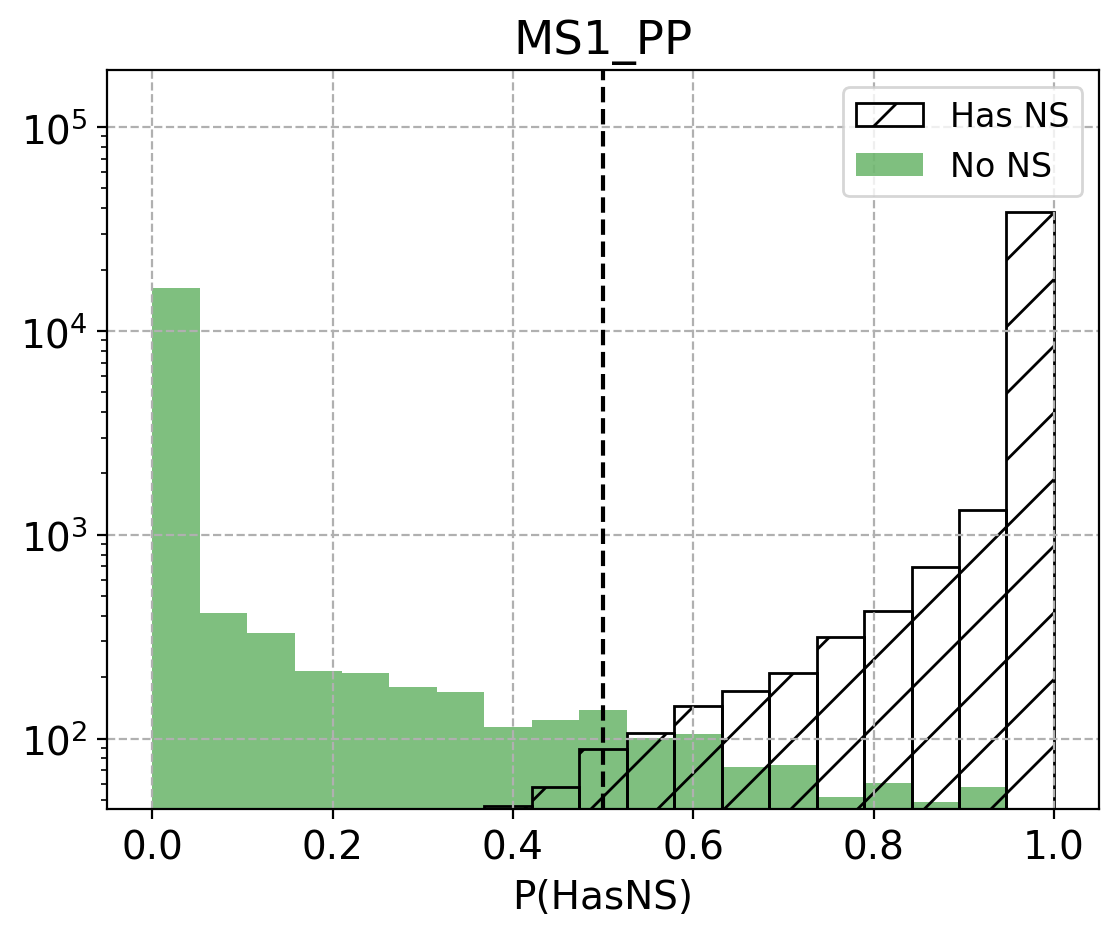
\includegraphics[width=0.45\textwidth]{/figs/MS1_PP_NShist}
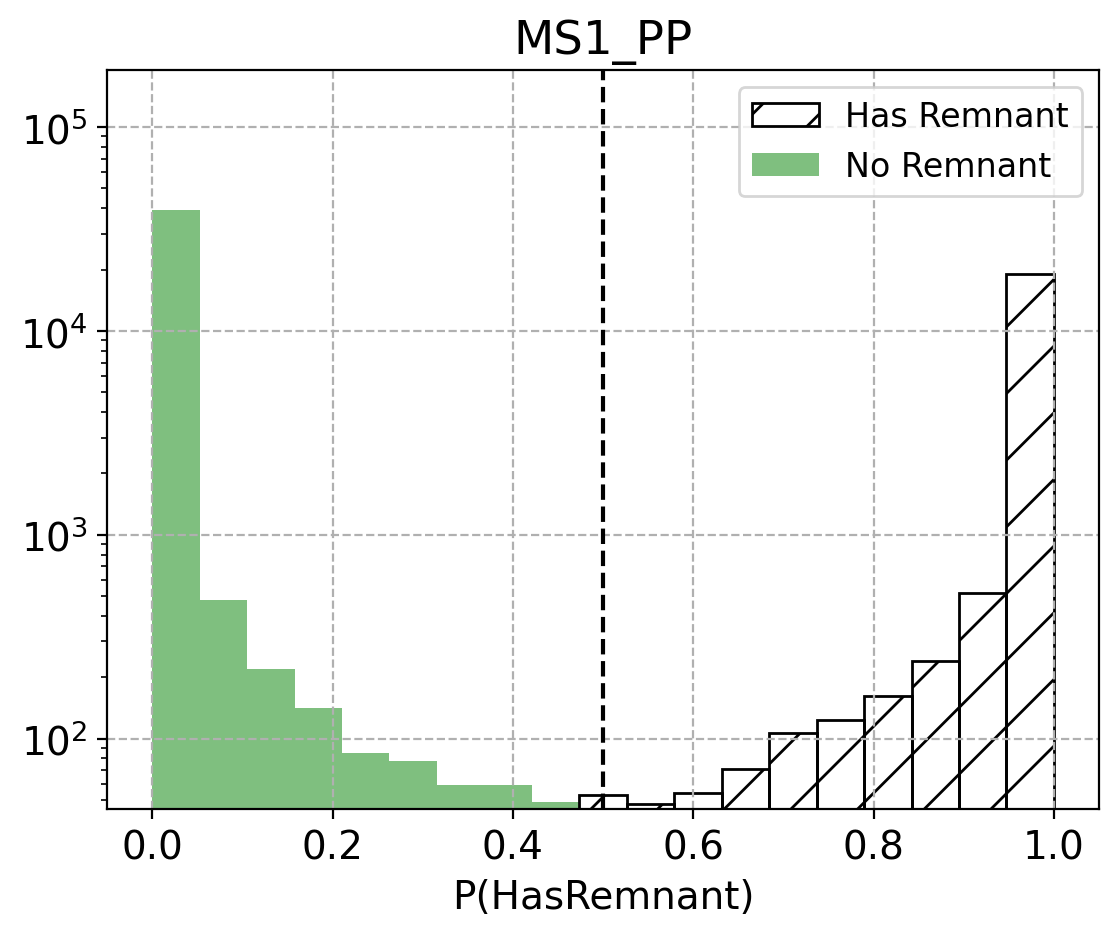
\includegraphics[width=0.45\textwidth]{/figs/MS1_PP_REMhist}
\caption{\label{fig:RF_hist_MS1PP} Histograms MS1 PP}
\end{figure}


 %plots and comments
%\input{GP_Results.tex}


%In order to decide which method gives a better performance in classifying this kind of events, we can apply them over testing data and finally do a comparison between both. A way to see how data is classified we can construct histograms where the number of events that are classified with a label (\texttt{HasNS/HasRemnant}) \texttt{True} or \texttt{False} will change with a given threshold of the probability. For an algorithm with perfect performance, all the events with label \texttt{True (False)} should be at \textit{p}(\texttt{label}) = 1 (\textit{p}(\texttt{label}) = 0).

%Another way to check the algorithm's performance is by building the so-called \textit{Receiver Operating Characteristic (ROC) Curve}. They show the variation of the true-positive rate (or efficiency) with the false-positive rate given a certain threshold for the probability. An algorithm with a proper performance will give a steeper ROC curve, or in other words, will have a higher eficiency with a lower false-positive rate.  


%In the ROC curves that we will present in the following subsections, we highlight three reference EoS in color, from which we show results in more detail. We select BHF\_BBB2 because is the model that give the lowest maximum mass, MS1\_PP as the model with the bigger maximum mass, and we also include SLy because is the most accepted EoS for NS modeling (reference), and is the one that was used in the injections that are our dataset.


%\subsection{Algorithm comparison}


%Here we talk about overall results and specifically from each algorithm in the
%subsections below.  \mmt{[MMT: Below I described how to check the performance of the algorithms. Maybe a table with all the scores/sensitivities/precisions from both %KNN and RF would be useful (already got it in a google doc)]}

%\mmt{To measure the performance of the classifiers we use some common statistical quantities.  The score is the number of correctly predicted events over the number %of total events (a perfect classifier has a score of 1).  It works best when there is an equal number of events for each label in the training set. It does not %consider the importance of misclassification, or that the training data can be biased towards one specific label.}

%\mmt{The mean score is computed by training the algorithm on the $90\%$ of the dataset and testing it on the remaining $10\%$, cycling the train/test combination over %the full dataset. To do that, we are going to use the training dataset, since it's the larger one.  In order to train and test the model and create the different %plots, we are going to use the training and testing files. }

%\mmt{Another useful quantity is the sensitivity. It is the ratio between the true positives and the sum of the true positives and false negatives.  It measures how %much the algorithm predicts \textit{true} (in our case it would be that the event has NS or has REM), when it is actually \textit{true}.Having a sensitivity equal to %1 would mean that our method predicts \textit{true} for every event. Therefore, a method with high sensitivity will barely miss true alarms. }

%\mmt{A quantity that measures how much you can trust a method when it predicts \textit{true} is the precision.  It is the ratio between the true positives and the %some of the true  and the false positives. A precision equal to 1 means that the method never predicts \textit{true} when it is actually \textit{false}. This means %that the method will never give false alarms. }

%\mmt{Finally, the F1 score $F1 = 2(\rm{precision \times sensitivity})/(\rm{precision+sensitivity})$ is a type of score that takes into consideration how precision and %sensitivity compensate each other. A perfect classifier would have a F1 score of 1.}

%To compare quantitatively the results from RF and KNN we compute the true positive and false positive rate for several threshold values, for both HasNS and HasREM, for the three selected EoS. These are tables \ref{tab:TPbhf}, \ref{tab:TPms1} and \ref{tab:TPsly}. For HasNS the two algorithms perform similarly, with almost the same TP for all threshold values and accross EoSs, although the false positive is smaller always in the RF. For HasREM we obtain that RF performs better than KNN in every case, with not only a smaller false positive rate, but a greater true positive rate.

%\begin{table}[]
%\centering
%\begin{tabular}{@{}c|cccc|cccc@{}}
%\toprule
%\multicolumn{1}{l|}{}          & \multicolumn{4}{c|}{Has NS}                       & \multicolumn{4}{c}{Has REM}                      \\ \midrule
%                               & \multicolumn{2}{c}{RF} & \multicolumn{2}{c|}{KNN} & \multicolumn{2}{c}{RF} & \multicolumn{2}{c}{KNN} \\
%\multicolumn{1}{l|}{Threshold} & TP         & FP        & TP          & FP         & TP         & FP        & TP         & FP         \\ \midrule
%0.1                            & 0.999      & 0.107     &   0.999          &  0.156          & 0.998      & 0.011     &    0.992        &  0.051          \\
%0.3                            & 0.998      & 0.068     &   0.996        &  0.117          & 0.993      & 0.005     &   0.974         &  0.017          \\
%0.5                            & 0.994      & 0.042     &   0.991          &  0.088           & 0.985      & 0.003     &   0.937         &  0.006          \\
%0.8                            & 0.967      & 0.014     &   0.966          & 0.043            & 0.957      & 0.001     &  0.845          &   0.001         \\ %\bottomrule
%\end{tabular}
%\caption{BHF\_BB2}
%\label{tab:TPbhf}
%\end{table}


%\begin{comment}
\begin{table}[]
\begin{tabular}{c|c|ccr|ccr}
\hline
\multicolumn{1}{c|}{}         & \multicolumn{1}{l|}{} & \multicolumn{3}{c|}{p(HasNS)}                                                & \multicolumn{3}{c}{p(HasREM)}                                                \\ \hline
\multicolumn{1}{c|}{event ID} & grace\_id             & \multicolumn{1}{c}{RF} & \multicolumn{1}{c}{KNN} & \multicolumn{1}{c|}{GP} & \multicolumn{1}{c}{RF} & \multicolumn{1}{c}{KNN} & \multicolumn{1}{c|}{GP} \\ \hline
GW170823                      & G298936               & 0.000                   & 0.000                    & 0.014                   & 0.000                   & 0.000                    & 0.001                   \\
GW170817                      & G298048               & 1.000                   & 1.000                    & 0.999                   & 1.000                   & 1.000                    & 0.995                   \\
GW170814                      & G297595               & 0.000                   & 0.000                    & 0.013                   & 0.000                   & 0.000                    & 0.001                   \\
GW170809                      & G296853               & 0.002                   & 0.000                    & 0.013                   & 0.000                   & 0.000                    & 0.001                   \\
GW190408                      & G329243               & 0.000                   & 0.000                    & 0.013                   & 0.000                   & 0.000                    & 0.001                   \\
GW190412                      & G329483               & 0.000                   & 0.000                    & 0.021                   & 0.000                   & 0.000                    & 0.001                   \\
GW190413-052954               & G329577               & 0.000                   & 0.000                    & 0.013                   & 0.000                   & 0.000                    & 0.001                   \\
GW190413-134308               & G329615               & 0.000                   & 0.000                    & 0.010                   & 0.000                   & 0.000                    & 0.001                   \\
GW190421                      & G330300               & 0.000                   & 0.000                    & 0.017                   & 0.000                   & 0.000                    & 0.001                   \\
GW190425                      & G330564               & 1.000                   & 1.000                    & 0.999                   & 0.999                   & 1.000                    & 0.994                   \\
GW190426                      & G330687               & 0.996                   & 1.000                    & 0.980                   & 0.009                   & 0.000                    & 0.008                   \\
GW190503                      & G331315               & 0.000                   & 0.000                    & 0.032                   & 0.000                   & 0.000                    & 0.001                   \\
GW190512                      & G332169               & 0.000                   & 0.000                    & 0.014                   & 0.000                   & 0.000                    & 0.001                   \\
GW190513                      & G332333               & 0.000                   & 0.000                    & 0.014                   & 0.000                   & 0.000                    & 0.001                   \\
GW190517                      & G333132               & 0.000                   & 0.000                    & 0.010                   & 0.000                   & 0.000                    & 0.001                   \\
GW190519                      & G333443               & 0.000                   & 0.000                    & 0.014                   & 0.000                   & 0.000                    & 0.001                   \\
GW190521-074359               & G333664               & 0.000                   & 0.000                    & 0.013                   & 0.000                   & 0.000                    & 0.001                   \\
GW190602                      & G335015               & 0.000                   & 0.000                    & 0.061                   & 0.000                   & 0.000                    & 0.001                   \\
GW190630                      & G337426               & 0.000                   & 0.000                    & 0.014                   & 0.000                   & 0.000                    & 0.001                   \\
GW190706                      & G337919               & 0.015                   & 0.000                    & 0.019                   & 0.000                   & 0.000                    & 0.001                   \\
GW190707                      & G337978               & 0.000                   & 0.000                    & 0.096                   & 0.000                   & 0.000                    & 0.001                   \\
GW190708                      & G338125               & 0.000                   & 0.002                    & 0.070                   & 0.000                   & 0.000                    & 0.001                   \\
GW190720                      & G344653               & 0.004                   & 0.000                    & 0.024                   & 0.000                   & 0.000                    & 0.001                   \\
GW190727                      & G345173               & 0.011                   & 0.000                    & 0.013                   & 0.000                   & 0.000                    & 0.001                   \\
GW190728                      & G345315               & 0.000                   & 0.000                    & 0.013                   & 0.000                   & 0.000                    & 0.001                   \\
GW190814                      & G347305               & 0.098                   & 0.647                    & 0.878                   & 0.000                   & 0.000                    & 0.002                   \\
GW190828-063405               & G348500               & 0.002                   & 0.000                    & 0.014                   & 0.000                   & 0.000                    & 0.001                   \\
GW190828-065509               & G348519               & 0.001                   & 0.000                    & 0.019                   & 0.000                   & 0.000                    & 0.001                   \\
GW190915                      & G350491               & 0.000                   & 0.000                    & 0.009                   & 0.000                   & 0.000                    & 0.001                   \\
GW190924                      & G351423               & 0.037                   & 0.075                    & 0.100                   & 0.000                   & 0.000                    & 0.001                   \\
GW190930                      & G351993               & 0.000                   & 0.000                    & 0.079                   & 0.000                   & 0.000                    & 0.001                   \\
GW191109                      & G354231               & 0.000                   & 0.000                    & 0.036                   & 0.000                   & 0.000                    & 0.001                   \\
GW191129                      & G355916               & 0.004                   & 0.000                    & 0.024                   & 0.000                   & 0.000                    & 0.001                   \\
GW191204-171526               & G356500               & 0.000                   & 0.000                    & 0.026                   & 0.000                   & 0.000                    & 0.001                   \\
GW191215                      & G357403               & 0.000                   & 0.000                    & 0.017                   & 0.000                   & 0.000                    & 0.001                   \\
GW191216                      & G357490               & 0.000                   & 0.000                    & 0.125                   & 0.000                   & 0.000                    & 0.001                   \\
GW191222                      & G358088               & 0.000                   & 0.000                    & 0.028                   & 0.000                   & 0.000                    & 0.001                   \\
GW200112                      & G359994               & 0.000                   & 0.000                    & 0.015                   & 0.000                   & 0.000                    & 0.001                   \\
GW200115                      & G360364               & 0.997                   & 1.000                    & 0.987                   & 1.000                   & 0.000                    & 0.011                   \\
GW200129                      & G361581               & 0.000                   & 0.000                    & 0.015                   & 0.000                   & 0.000                    & 0.001                   \\
GW200219                      & G364596               & 0.000                   & 0.000                    & 0.027                   & 0.000                   & 0.000                    & 0.001                   \\
GW200224                      & G365371               & 0.014                   & 0.000                    & 0.027                   & 0.000                   & 0.000                    & 0.001                   \\
GW200225                      & G365427               & 0.001                   & 0.000                    & 0.013                   & 0.000                   & 0.000                    & 0.001                   \\
GW200302                      & G366190               & 0.000                   & 0.000                    & 0.014                   & 0.000                   & 0.000                    & 0.001                   \\
GW200311                      & G367788               & 0.000                   & 0.000                    & 0.01                    & 0.000                   & 0.000                    & 0.001                   \\
GW200316                      & G368545               & 0.000                   & 0.000                    & 0.068                   & 0.000                   & 0.000                    & 0.001                   \\
GW200322                      & G369200               & 0.012                   & 0.000                    & 0.031                   & 0.000                   & 0.000                    & 0.001                   \\ \cline{1-1} \cline{3-4} \cline{6-7}
\hline
\end{tabular}
\caption{PROBAB TABLE REAL DATA - from algo. Update to marginalized bayesian or remove.}
\label{tab:real_data}
\end{table}
%\end{comment}

%\begin{comment}
\begin{table}[]
\begin{tabular}{c|c|cc|cc}
\hline
\multicolumn{1}{c|}{}         & \multicolumn{1}{l|}{} & \multicolumn{2}{c|}{$P(\hasns)$}                                                & \multicolumn{2}{c}{$P(\hasrem)$}                                                \\ \hline
\multicolumn{1}{c|}{event ID} & grace\_id             & \multicolumn{1}{c}{RF} & \multicolumn{1}{c}{KNN}  & \multicolumn{1}{c}{RF} & \multicolumn{1}{c}{KNN} \\ \hline
GW170817                      & G298048               & 1.000                   & 1.000                    & 1.000                   & 1.000                                  \\
GW190425                      & G330564               & 1.000                   & 1.000                    & 0.999                   & 1.000                             \\
GW190426                      & G330687               & 0.996                   & 1.000                    & 0.009                   & 0.000                     \\
GW190814                      & G347305               & 0.098                   & 0.647                    & 0.000                   & 0.000                      \\
GW190924                      & G351423               & 0.037                   & 0.075                    & 0.000                   & 0.000                       \\               
GW200115                      & G360364               & 0.997                   & 0.987                   & 0.006                   & 0.000                           \\
\hline
\end{tabular}
\caption{Short table with probabilities (from algo) for O3 real events. I don't think we want this anymore. \mmt{[MMT: we can remove, let's see what Marco thinks.]}}
\label{tab:real_data_short}
\end{table}
%\end{comment}



